\documentclass[11pt,a4paper]{article}
\usepackage[margin=2.5cm]{geometry}
\usepackage[T1]{fontenc}
\usepackage{lmodern}
\usepackage{longtable}
\usepackage{booktabs}
\usepackage{enumitem}
\usepackage[hidelinks]{hyperref}
\usepackage{xcolor}
\usepackage{graphicx}

\newcommand{\done}{\textcolor{green!45!black}{\textbf{Done}}}
\newcommand{\pending}{\textcolor{blue!60!black}{\textbf{Built, mining target not achieved yet}}}
\newcommand{\partialx}{\textcolor{orange!80!black}{\textbf{Partial}}}
\newcommand{\gap}{\textcolor{red!70!black}{\textbf{Gap}}}
\newcommand{\code}[1]{\texttt{\detokenize{#1}}}
\setlist{itemsep=2pt,topsep=4pt}
\setlength{\parskip}{4pt}
\setlength{\parindent}{0pt}
\setlength{\emergencystretch}{3em}

\definecolor{rifflecolor}{HTML}{27187E}
\newcommand{\handle}[1]{{\small\texttt{#1}}}

\begin{document}
\thispagestyle{empty}
\vspace*{0.26\textheight}
\begin{center}

\includegraphics[width=0.52\textwidth]{figures/riffle_logo.pdf}\\[1.6em]
{\large\itshape Every repo breaks differently.}\\[7em]
{\Large Data Pipeline Report}\\[0.8em]
{\normalsize DADS 7305 $\bullet$ Machine Learning Operations}
\end{center}
\vfill
\begin{center}
{\small October 2026}
\end{center}
\clearpage

\thispagestyle{empty}
{\Large\bfseries\color{rifflecolor} Team}\\[2.2em]
\begin{tabular}{@{}p{4.2cm}l@{}}
Rudr & \handle{ru-dr}\\[0.55em]
Divyam Patel & \handle{Divyam2701}\\[0.55em]
Nishit Chaudhary & \handle{nishit3}\\[0.55em]
Naman Lazarus & \handle{23daVinci}\\[0.55em]
Ananth T A & \handle{ananth-ta}\\[0.55em]
Preeyal Jadhav & \handle{preeyaljadhav}\\
\end{tabular}

\vspace{3.2em}
\begin{tabular}{@{}p{2.6cm}l@{}}
Repository & \href{https://github.com/ru-dr/riffle}{\textcolor{rifflecolor!80}{\texttt{https://github.com/ru-dr/riffle}}}\\[0.55em]
Live site & \href{https://rifffle.vercel.app}{\textcolor{rifflecolor!80}{\texttt{https://rifffle.vercel.app}}}\\
\end{tabular}
\clearpage

\begin{abstract}
Riffle is a self-hosted GitHub App that ranks pull requests (PRs) by learned risk. This report describes its data pipeline against the course guidelines: acquisition, preprocessing, tests, Airflow orchestration, DVC versioning, logging, schema and statistics, anomaly alerts, flow optimisation and bias detection by data slicing. Each item is marked \done; \pending, meaning the mechanism is built and tested and the mining target (all planned PRs mined) is not achieved yet, so its final evidence is still to come; \partialx, meaning a piece is not built; or \gap. Open pieces are stated, not hidden. Bias numbers come from one data shard and should be refreshed on the merged tables before submission.
\end{abstract}

\tableofcontents
\newpage

%--------------------------------------------------------------------
\section{Overview}

The pipeline turns GitHub PR history into three training tables. They have different grains, so they are kept apart and joined at load time by \code{pipelines/training/frames.py}.

\begin{center}
\begin{tabular}{@{}lll@{}}
\toprule
Table & Grain & Contract \\
\midrule
dataset & one row per closed PR & \code{mined_dataset} \\
snapshots & one row per PR moment while open & \code{mined_snapshot} \\
commit features & one row per head commit & \code{mined_commit_features} \\
\bottomrule
\end{tabular}
\end{center}

Two sources feed it:
\begin{enumerate}
  \item \textbf{Repo miner} (\code{pipelines/ingestion/repo_miner/}): clones repositories, calls the GitHub API, computes labels and features.
  \item \textbf{AIDev} (\code{pipelines/ingestion/aidev/}): a pinned Hugging Face dataset of PRs opened by AI coding agents. It is used as a detector test set and a taxonomy source, not as training data (section~\ref{sec:aidev}).
\end{enumerate}

Data flow:
\begin{enumerate}[label=\arabic*.]
  \item GitHub API and git clones $\rightarrow$ miner stages $\rightarrow$ \code{merge_shards.py}.
  \item \code{publish.py check} (contracts) $\rightarrow$ \code{publish.py push} (DVC) $\rightarrow$ \code{frames.py}.
  \item AIDev (Hugging Face) $\rightarrow$ download, verify, upload to GCS $\rightarrow$ test set for the agent detector (not joined into training frames).
\end{enumerate}

\section{Miner Flow Diagrams}\label{sec:flow}

Three diagrams show how the miner works, from the whole batch down to one pull request. They follow \code{ARCHITECTURE.md} and \code{stages.py}. Where the two differ, the code is right: \code{stages.py} lists 13 per-repository stages, including \texttt{reviews prefetch}, which the architecture table omits.

\subsection{End to end}
Figure~\ref{fig:flow1} shows what runs on each PC and what happens after. The batch driver reads the repos file, keeps this PC's share and mines one repository at a time in its own subprocess, so a crash loses at most that repository's unfinished work, and the checkpoint lets a rerun resume. After every repository the PC sends its logs, health files and tables to the team store. After the batch, the PCs' files are merged, checked against the contracts, versioned with DVC and read by the training loader.

\begin{figure}[!htbp]
\centering
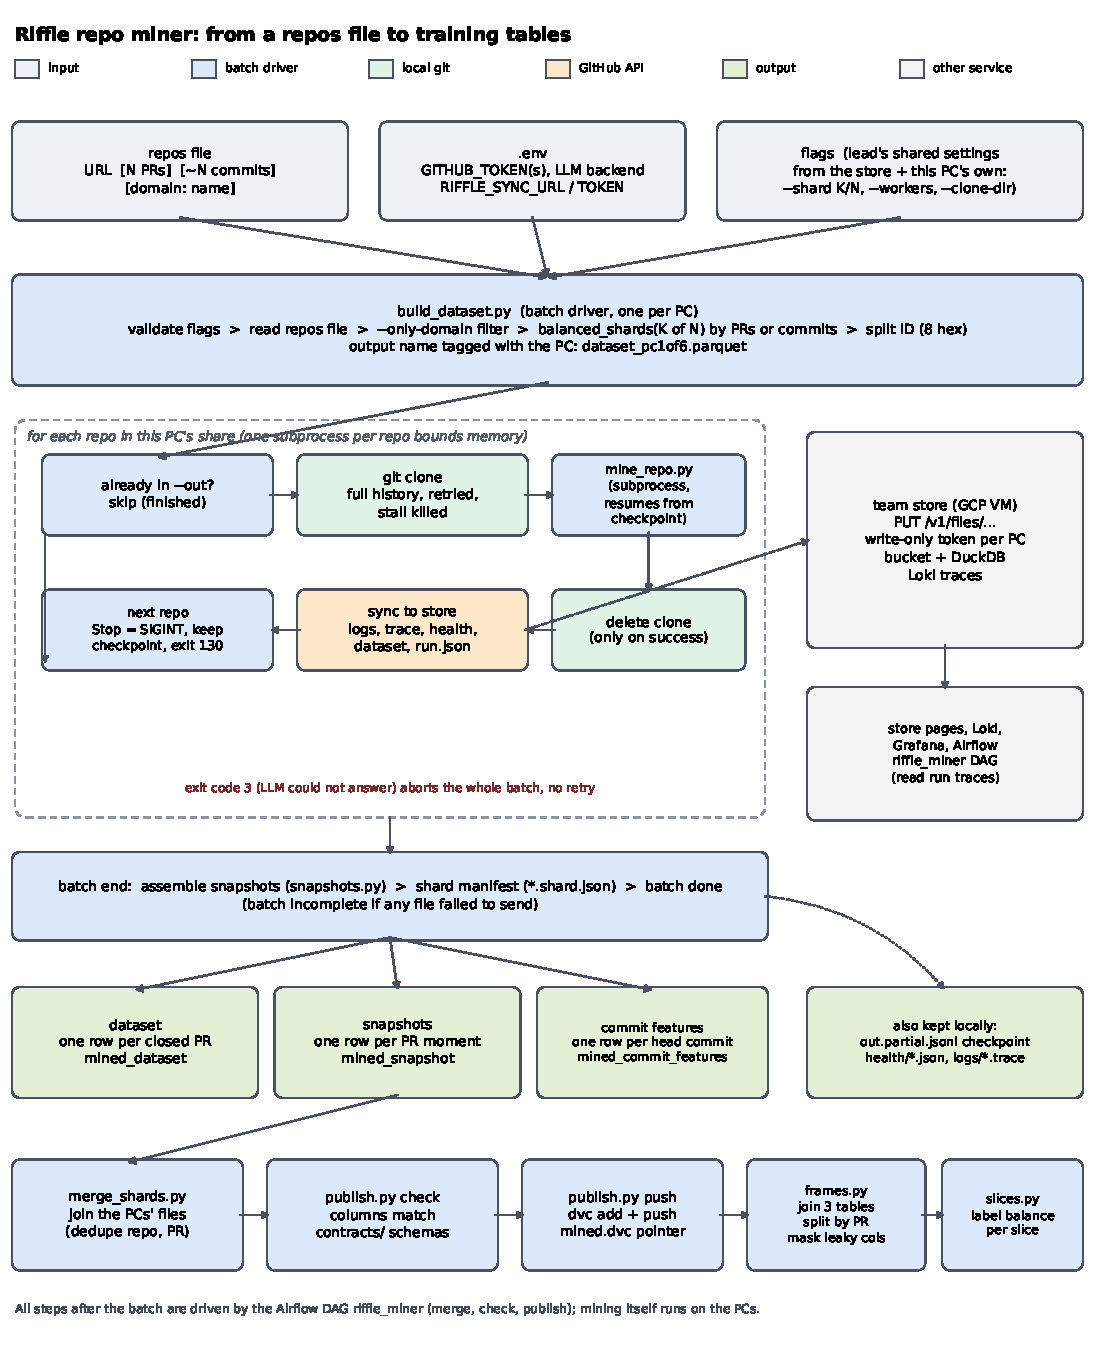
\includegraphics[width=0.96\textwidth]{figures/flow_miner_overview.pdf}
\caption{End-to-end flow of the miner: inputs, batch driver, the per-repository loop, outputs and the steps after mining.}
\label{fig:flow1}
\end{figure}

\subsection{One repository}
Figure~\ref{fig:flow2} lists the stages \code{mine_repo.py} runs, in order, and what each one calls. Stages in orange depend on the GitHub API and are bound by its rate limits. Stages in green read the local clone. The clone is full-history, never shallow, because history features and SZZ need the commits before each PR.

\begin{figure}[!htbp]
\centering
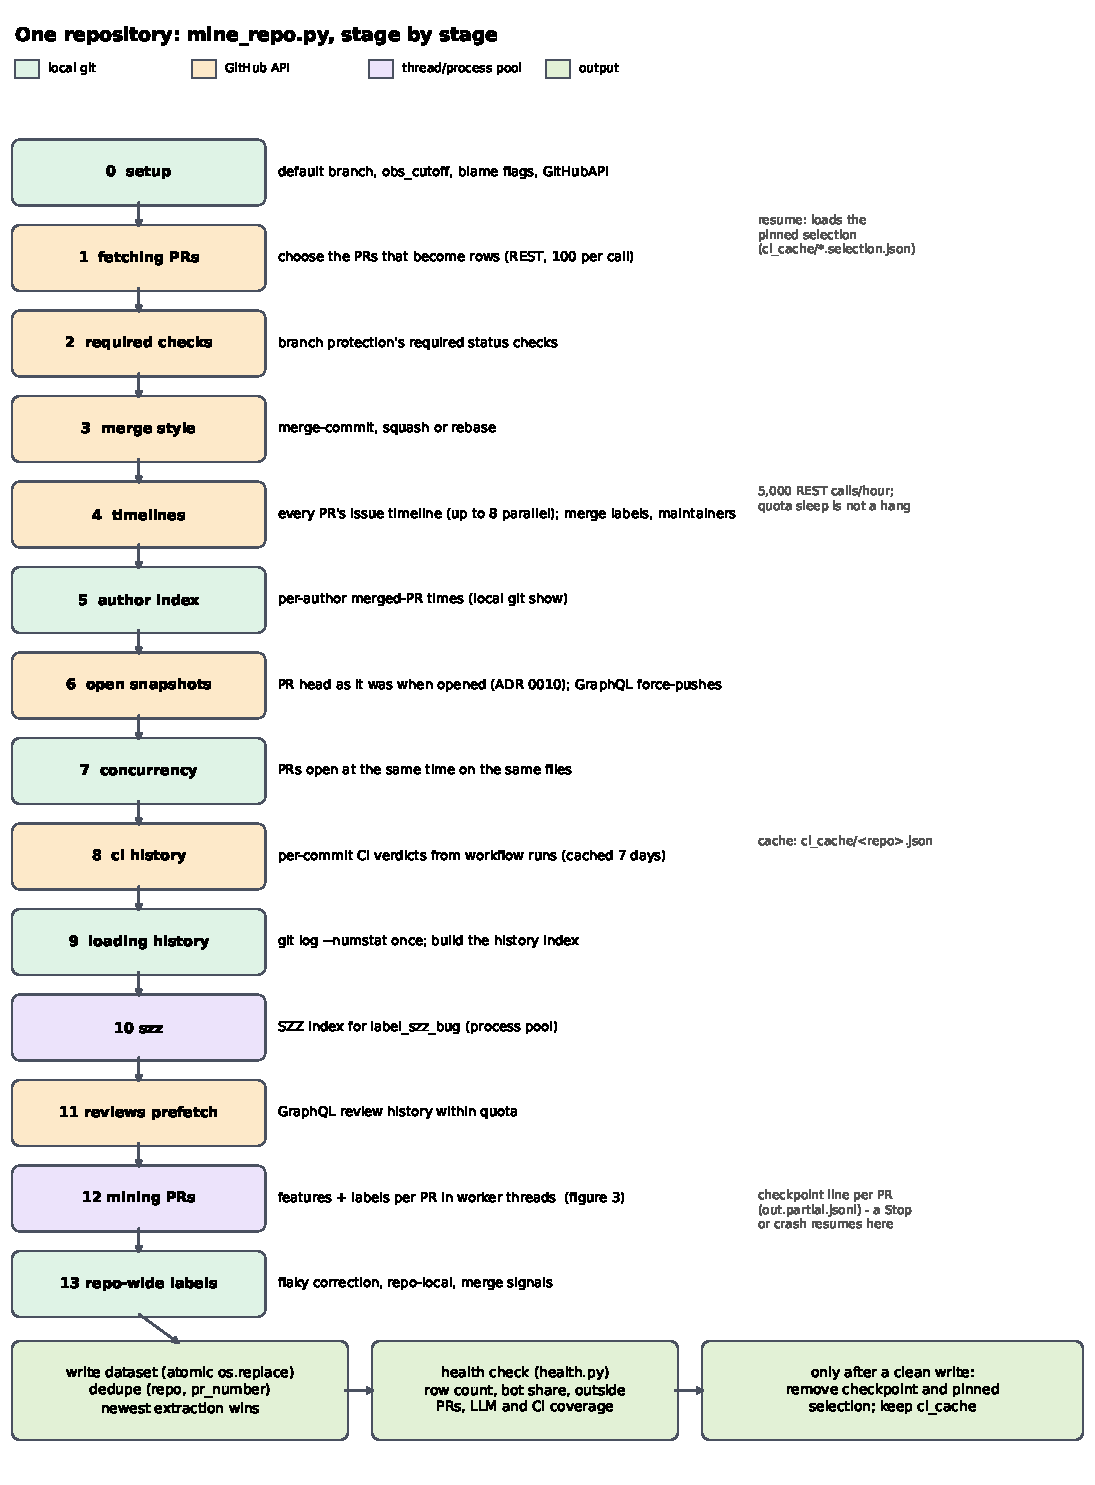
\includegraphics[width=0.9\textwidth]{figures/flow_miner_repo.pdf}
\caption{The per-repository stages of \code{mine_repo.py}. The Airflow DAG draws one node per stage.}
\label{fig:flow2}
\end{figure}

\subsection{One pull request}
Figure~\ref{fig:flow3} shows how one PR becomes one row. Features are computed from the PR as it stood when it opened and from history before its fork point. Only the labels look forward, using the final range of the PR. The workers run in parallel, but a single consumer takes results in PR order, so a rerun produces the same file whatever the thread timing.

\begin{figure}[!htbp]
\centering
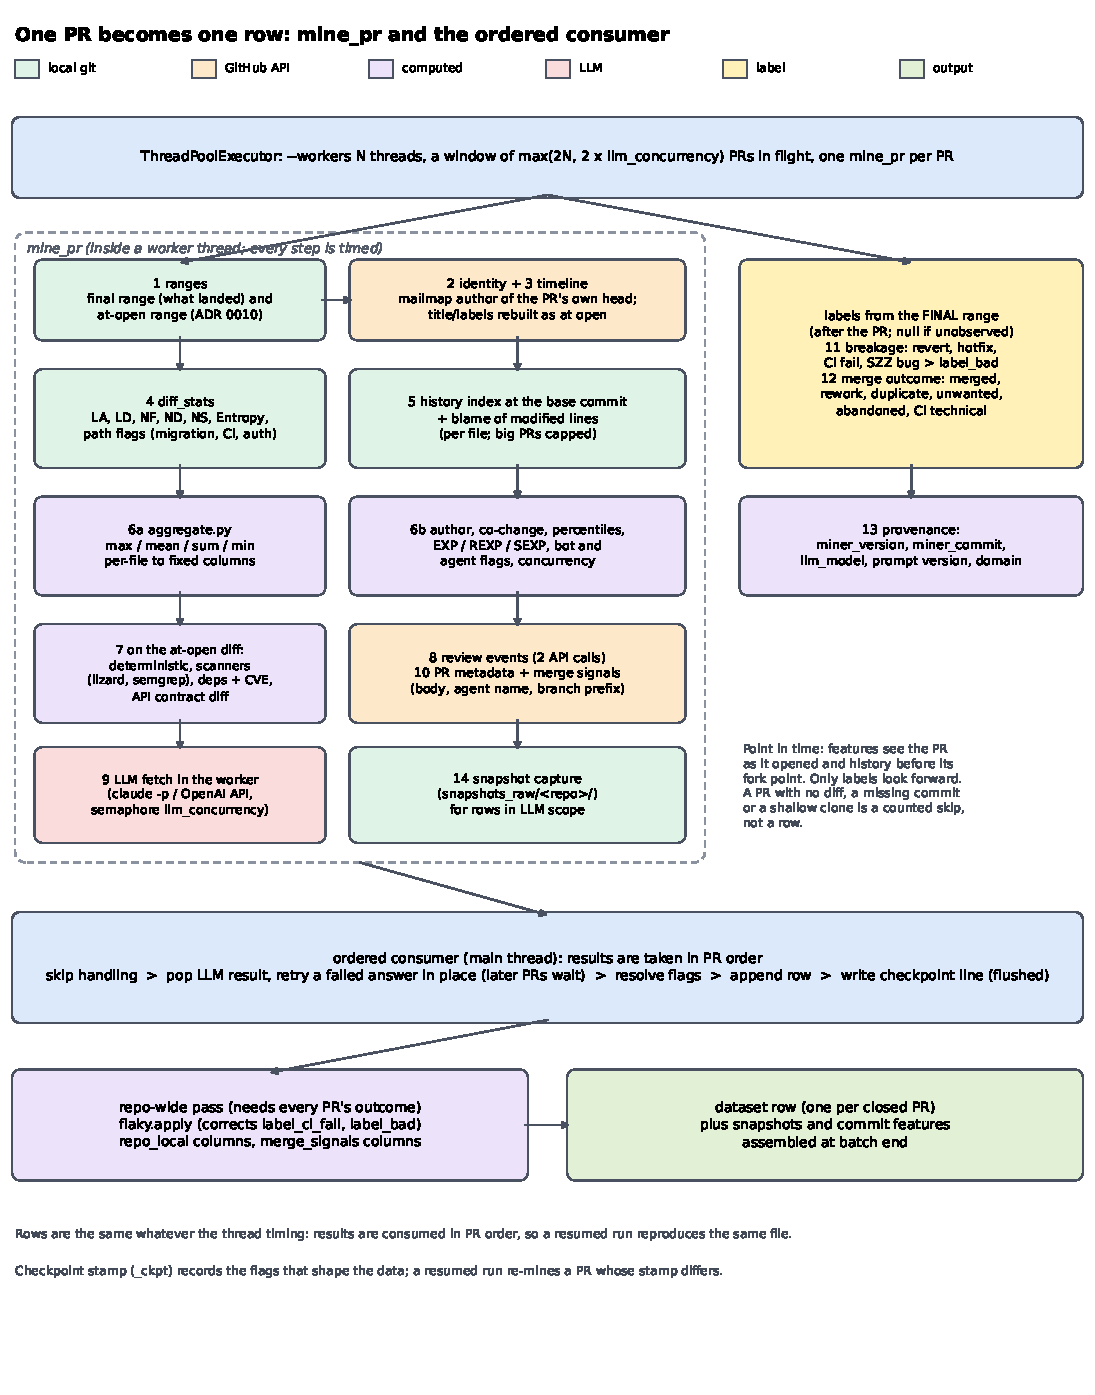
\includegraphics[width=0.9\textwidth]{figures/flow_miner_pr.pdf}
\caption{Inside \code{mine_pr}, and the ordered consumer that writes the row and its checkpoint line.}
\label{fig:flow3}
\end{figure}

\subsection{The same flow in Airflow}
The DAG draws the per-repository stages as a task group. Figure~\ref{fig:dagbig} is the graph view of the test run in section~\ref{sec:testrun} with the group expanded: a chain of stage tasks, the \texttt{pr\_*} steps in parallel with \texttt{mining\_prs}, then \texttt{repo\_wide\_labels}, \texttt{gate}, \texttt{gather}, \texttt{merge}, \texttt{check} and \texttt{publish}.

\begin{figure}[!htbp]
\centering
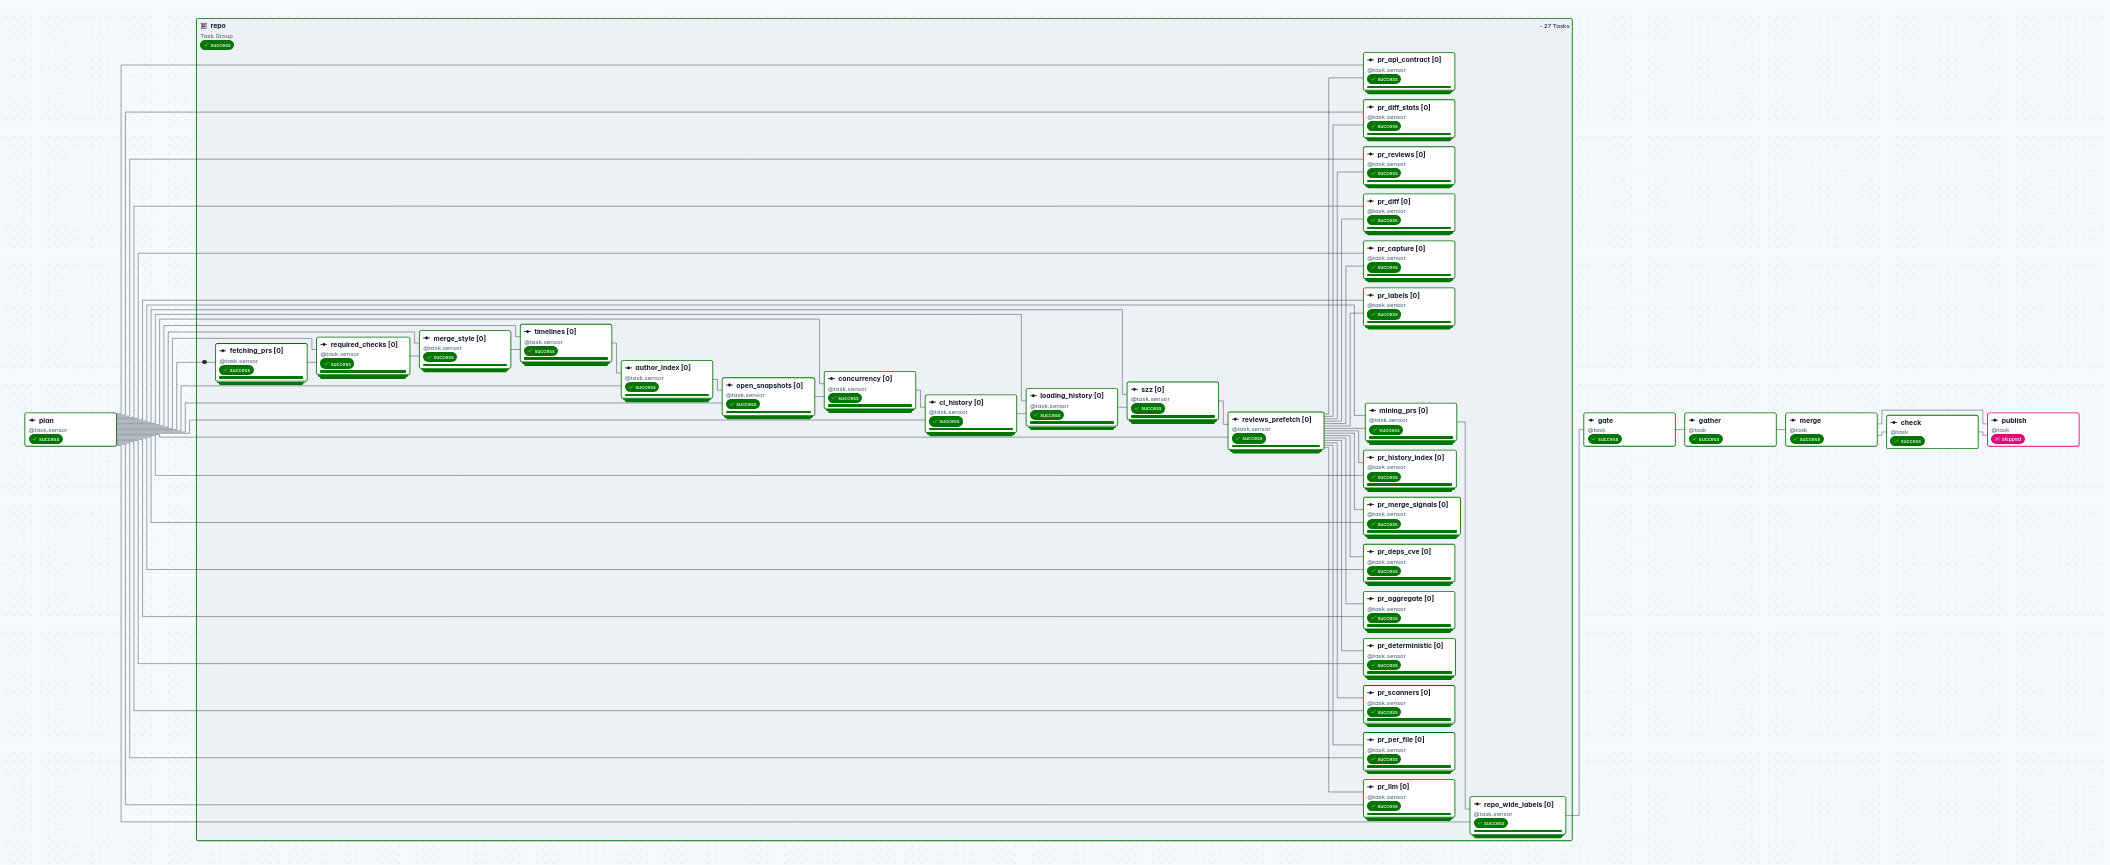
\includegraphics[width=\textwidth]{figures/dag_graph_expanded.png}
\caption{Airflow graph view of \code{riffle_miner} with the \texttt{repo} task group expanded (27 tasks per repository). Green nodes succeeded; \texttt{publish} was skipped.}
\label{fig:dagbig}
\end{figure}

%--------------------------------------------------------------------
\section{Why We Run Our Own Miner, and What Public Datasets Lack}\label{sec:aidev}

AIDev is a useful public dataset, and the pipeline downloads and verifies it. We use it for two things only: a test set for our agent detector and a source for the agent taxonomy. We do not train on it. The reasons are below. Some facts come from our pin (\code{aidev/aidev_ingest/pin.py}), the proposal, the data-management plan and ADR 0009; the label and skew arguments are our own analysis.

\subsection{What AIDev is good for}
\begin{itemize}
  \item \textbf{Agent names, login patterns and 11 task categories.} These are a good reference for our agent detector (\code{ai_agent_authored}, \code{agent_name}). Its PRs, where the author is known to be an agent, make a test set to measure the detector's precision and recall.
  \item \textbf{A pinned, verified snapshot.} The pin is a commit hash and every file is checked by SHA-256, so the test set cannot change under us.
\end{itemize}

\subsection{Why we do not train on it}
\begin{enumerate}
  \item \textbf{The label is not risk.} Merged versus not merged is a maintainer decision. AIDev has no revert, hotfix or SZZ labels, which are what Riffle's breakage target (\code{label_bad}) needs.
  \item \textbf{Closed PRs are noisy.} Many closed agent PRs reflect a maintainer's policy about AI, not the quality of the code. That adds noise to a merge label.
  \item \textbf{The agent name becomes a shortcut.} A model could learn ``Copilot means rejected'' instead of ``this change is risky''. A feature that stands in for the label is a bias we cannot afford.
  \item \textbf{Only agent PRs.} Riffle must rank every PR, including human and outside-contributor PRs. A model trained only on agent PRs may fail on human ones. ADR 0009 states that training data comes from the miner's own mining and that AIDev is not ingested.
  \item \textbf{It is a snapshot.} We cannot rebuild point-in-time features at each PR's base commit without mining the repositories ourselves. The plan already hydrates contributor status, CI state and timestamps from the GitHub API for this reason.
  \item \textbf{It does not pass through our miner.} Training and serving would use different feature code, which causes train/serve skew.
  \item \textbf{Cut-off and coverage.} The pinned revision ends on 2026-03-31, and it covers only repositories with more than 100 stars in its ``pop'' tables. The large commit-details table is written without its \code{patch} column, and \code{pr_review_comments} is held back, because both carry code from repositories with mixed licences.
\end{enumerate}

\subsection{Other datasets we considered, and why each falls short}
AIDev is not the only candidate. The project proposal and the data-management plan name several more. None of them gives Riffle what it needs: real PRs, features rebuilt as the PR stood when it opened, and breakage labels that look forward. Table~\ref{tab:datasets} lists them with the reason each lacks something. Sizes and roles come from the proposal; the reasons marked with an asterisk are our reading of what each dataset contains and should be checked against its documentation.

\begin{center}
\small
\begin{longtable}{@{}p{2.9cm}p{4.4cm}p{7.3cm}@{}}
\caption{Public datasets considered for Riffle and why each is not enough on its own.}\label{tab:datasets}\\
\toprule
Dataset & What it is & Why it lacks \\
\midrule
\endfirsthead
\toprule
Dataset & What it is & Why it lacks \\
\midrule
\endhead
AIDev & agent PRs from six agents; 33,596 PRs from 2,807 popular repositories in the pop subset; cut-off 2026-03-31 in our pin & Agent PRs only, popular repositories only, no breakage labels, a snapshot we cannot rebuild point-in-time features from, and a fixed cut-off (section above). \\
MOSAIC-agentic-3m & 111,969 agent and human PRs, June to August 2025 & Covers only three months, so it cannot show drift or long history. Its licence is still an open question in our plan. It has a human baseline, which AIDev lacks, but no revert, hotfix or SZZ labels,* and no features at the PR's base commit.* \\
Hand-coded rejection sets (Ehsani et al.; Peralta et al.) & about 600 and 717 PRs, coded by people for why agent PRs were rejected & Far too small to train on (hundreds of PRs), agent PRs only, and they hold labels without our features. Our plan uses them to seed the label taxonomy and to validate our labeller, not for training. \\
DupPR & 2,323 duplicate PR pairs & Built for one task, finding duplicate pairs. It has no merge outcome or breakage label for a single PR, so it can only train the duplicate-similarity feature.* \\
AgenticFlict & 107,026 simulated PRs, 27.7\% with merge conflicts & The PRs are simulated, so the outcome is a conflict in a replay, not a maintainer's decision or a breakage after merge. It can add a conflict feature at most. \\
ApacheJIT & just-in-time defect data with SZZ bug-inducing labels on Apache projects & Its labels are SZZ labels, which are heuristic. Training and grading on the same heuristic is circular, which is why ADR 0002 reports it only alongside our own target. It covers Apache projects only, so it does not match the web ecosystem we mine.* \\
GH Archive on BigQuery & the public GitHub event stream & Since October 2025 GitHub trims the event payloads, so it can find candidate PRs but cannot describe them. It is a discovery index, not a training set. \\
SWE-bench-style benchmarks (METR, March 2026) & patches judged by whether tests pass & Passing tests is a weak proxy for merging: METR found maintainers' decisions about 24 points below automated grading. The label is not the maintainer's decision, and the patches are not real PRs from real contributors. \\
\bottomrule
\end{longtable}
\end{center}

\textbf{The common pattern.} Each dataset fixes one labelled question (merged or not, duplicate or not, conflict or not, test-passing or not) for a fixed set of PRs. Riffle needs one thing none of them provides: a breakage label (revert, hotfix, CI failure, SZZ) together with features rebuilt at the PR's base commit, for any repository we choose, as recent as we need. That combination only comes from mining the repositories ourselves. The public datasets still help as checks and seeds: AIDev and MOSAIC to test the agent detector, the hand-coded sets to validate the labeller, and DupPR to pre-train the duplicate feature.

\subsection{Why our own miner is a good approach}
\begin{itemize}
  \item \textbf{Full control of the data.} We choose the repositories (lists in \code{repos*.txt}, with domain tags), the PRs, the features and the labels. Nothing is limited to a third party's schema.
  \item \textbf{One code path.} Training and serving features come from the same miner code, so there is no train/serve skew.
  \item \textbf{Point-in-time by construction.} Features use the PR as it stood when it opened (ADR 0010) and history strictly before its fork point. Tests guard against leakage.
  \item \textbf{Honest labels.} We mine revert, hotfix, CI-failure and SZZ labels. An unobserved label stays null and is never counted as a pass. Slicing (section~\ref{sec:bias}) shows why: only 9.5\% of rows have an observed breakage label, and we can see that because we track it.
  \item \textbf{Contracts and versions.} Every table is checked against a JSON Schema, and every row records the miner version and commit. When a rule changes we bump the version and re-mine.
  \item \textbf{Fresh and repeatable.} New PRs can be mined as they appear, and a run can be repeated from its logged flags. Our shard holds PRs up to August 2026.
  \item \textbf{Own infrastructure and licence control.} Mining is sharded over six machines, progress goes to our own store, and tables are versioned with DVC. We keep derived features, not raw patches.
\end{itemize}

\subsection{Trade-offs}
Mining is slower and costs effort. GitHub rate limits and clone time mean a full run takes days on six machines, only some PCs have finished (section~\ref{sec:store}), and the breakage label needs time for its observation window to close. Our shard has only 129 AI-agent PRs, so the agent slice is thin. The answer is to mine more agent-authored PRs ourselves, using the detector that AIDev helps us test, and not to train on AIDev rows.

%--------------------------------------------------------------------
\section{Key Components}

\subsection[Data Acquisition]{Data Acquisition \hfill \done}
\begin{itemize}
  \item The miner (\code{github_api.py}, \code{gitio.py}, \code{api_cache.py}) fetches PRs, timelines, reviews and git history. A token pool and API limit handling keep it inside GitHub's rate limits. Repository lists are data (\code{repos*.txt}), not code.
  \item AIDev is pinned to a commit hash (\code{b37f9fd1...}, tag \code{v5}), not a tag that can move. \code{download.py} fetches 11 tables. \code{verify.py} checks each file's SHA-256 against the committed inventory \code{expected/aidev-v5.inventory.json}. \code{upload.py} copies the tables to a GCS raw bucket, verifies each object, then deletes the local copy.
  \item Dependencies are listed in \code{repo_miner/requirements.txt}, \code{aidev/pyproject.toml} and \code{infra/docker/airflow/requirements.txt}.
  \item Reproducible: \code{python -m aidev_ingest check} fails if the Hub no longer matches the pin.
\end{itemize}

\subsection[Data Preprocessing]{Data Preprocessing \hfill \done}
\begin{itemize}
  \item One module per concern: \code{labels.py}, \code{snapshots.py}, \code{aggregate.py}, \code{deps.py}, \code{flaky.py}, \code{maintainers.py}, \code{naming.py} and \code{features/}. Normalisation lives only in \code{pipelines/ingestion/}.
  \item An unobserved label stays null (\code{ci_observed}, \code{label_bad_observed}). Null is never treated as a pass.
  \item Features are point-in-time with no leakage. Two test files guard this:\\
  \code{test_history_leakage.py} and\\
  \code{test_deps_cve_point_in_time.py}.
  \item \code{merge_shards.py} and \code{merge_labels.py} combine shards from several machines.
\end{itemize}

\subsection[Test Modules]{Test Modules \hfill \done}
\begin{itemize}
  \item About 60 test files in \code{repo_miner/tests}, plus suites for \code{aidev}, \code{pipelines/training}, the Airflow scripts, the data store, the contracts and the logging stack. CI runs them.
  \item Edge cases covered by name: unobserved labels (\code{test_scanners_unobserved.py}), incomplete shards (\code{test_merge_shards_incomplete.py}), force-pushed history (\code{test_force_push_cache.py}), stale versions (\code{test_version_stale.py}), checkpoint resume (\code{test_checkpoint_resume.py}), LLM failures (\code{test_llm_failures.py}).
  \item The miner tests need no network, semgrep or LLM.
\end{itemize}

\subsection[Pipeline Orchestration (Airflow DAGs)]{Pipeline Orchestration (Airflow DAGs) \hfill \done}
\begin{itemize}
  \item \code{pipelines/dags/riffle_miner.py}: one sensor task per miner stage per repository (\code{fetching PRs}, \code{timelines}, \code{szz}, \code{mining PRs}, and so on), then \code{gate}, \code{gather}, \code{merge}, \code{check}, \code{publish}.
  \item Mining runs on team machines. The stage tasks read the run traces and show each stage's status, time and errors. The last tasks merge the shards, check them against \code{contracts/} and version them with DVC.
  \item Runs on Docker Compose (\code{infra/docker/airflow/}, ADR 0013). \code{riffle_smoke.py} checks the stack.
  \item Failure handling: sensors reschedule with a one-week timeout; \code{publish} fails on a remote outside the allow-list and skips when no remote is given.
\end{itemize}

\subsection[Data Versioning with DVC]{Data Versioning with DVC \hfill \pending}
\begin{itemize}
  \item \code{publish.py push} copies the merged tables and manifest into \code{mined/<miner_version>/}, runs \code{dvc add} and \code{dvc push} to a \code{gs://} remote, and writes the \code{mined.dvc} pointer. DVC uses the VM's service account, not a key file.
  \item The miner version (\code{version.py}) ties every table to the code that made it.
  \item The mechanism is tested end to end (section~\ref{sec:dvc}). The \code{data/mined.dvc} pointer is committed once the merged v7 tables exist, which happens once the mining target is achieved.
\end{itemize}

\subsection[Tracking and Logging]{Tracking and Logging \hfill \done}
\begin{itemize}
  \item \code{runlog.py} and \code{progress.py} write per-stage run traces; \code{trace_report.py} summarises them.
  \item Traces reach a shared Loki through the team store (ADR 0017) and are shown in Grafana. \code{infra/compose.logging.yaml} runs Loki, Alloy and Grafana locally. Airflow task logs add to this.
\end{itemize}

\subsection[Data Schema and Statistics Generation]{Data Schema and Statistics Generation \hfill \done}
\begin{itemize}
  \item The JSON Schemas in \code{contracts/} are the source of truth; \code{contracts/REFERENCE.md} is generated by \code{gen_reference.py}. Every change bumps \code{x-riffle-version} and adds a row to \code{docs/contracts.md}.
  \item CI checks that miner columns match the schemas in both directions, that rows validate, and that flat and nested forms convert losslessly (ADR 0012). \code{publish.py check} repeats the column check on each merged table before DVC.
  \item \code{health.py} summarises row counts, bot share, outside-contributor share and unobserved-CI share per repository.
  \item Statistics are produced by \code{health.py} per repository and shown live in the dashboards (section~\ref{sec:dash}). We validate with our own JSON Schema contracts, which CI enforces, instead of Great Expectations or TFDV. A per-run statistics file compared between runs is a possible addition.
\end{itemize}

\subsection[Anomaly Detection and Alerts]{Anomaly Detection and Alerts \hfill \done}
\code{health.py} flags a repository before it reaches training:

\begin{center}
\begin{tabular}{@{}ll@{}}
\toprule
Check & Threshold \\
\midrule
too few rows & fewer than 50 \\
unmerged outside-contributor PRs & under 5\% \\
bot PRs & over 50\% of rows \\
LLM columns missing & over 2\% of rows in scope \\
CI labels unobserved & over 80\% \\
\bottomrule
\end{tabular}
\end{center}

\code{publish.py check} fails the DAG on schema violations and on a miner-version mismatch.

Alerts reach people in four places: warnings in the TUI log, the same warnings in the web view and big picture, an \emph{offline} banner on the store's big picture when a PC stops syncing, and a failed \code{check} or \code{gate} task in Airflow (section~\ref{sec:dash}). The test run in that section shows two real flags: ``only 10 rows (< 50) and ``CI unobserved on 100\% of merged rows. Email or Slack delivery is not wired; the alerts are in the tools the team already watches.

\subsection[Pipeline Flow Optimisation]{Pipeline Flow Optimisation \hfill \pending}
Per-repository stage chains run in parallel in the DAG, mining is sharded across machines (\code{--shard K/N}), CI history is fetched in parallel windows, and stage results are cached and resume from checkpoints.

The Gantt view of a test run is captured and read in section~\ref{sec:testrun}. A demo this small cannot name a real bottleneck, so the same chart for the full run is added once the mining target is achieved.

\section{Test Run of the Pipeline}\label{sec:testrun}

To check the pipeline works, I ran it end to end on this machine on 27 October 2026. The Airflow stack from \code{infra/docker/airflow} was already up under Docker Compose. I triggered \code{riffle_miner} from the API for miner version 7.0.1 and split \texttt{45ea6f14}. This is a small demo run held in the local store: one repository (\texttt{pallets/itsdangerous}) and 12 PRs, so it finishes in seconds. Screenshots were taken with Firefox.

\textbf{Scope and limits.} The run follows a finished demo run from the store. It does not re-mine anything. The \code{publish} task was skipped on purpose because no \code{dvc_remote} was given. DVC was tested separately (section~\ref{sec:dvc}) against a local folder, not Google Cloud Storage, so it shows the mechanism, not the production remote.

\subsection{Airflow DAG}
\begin{figure}[!htbp]
\centering
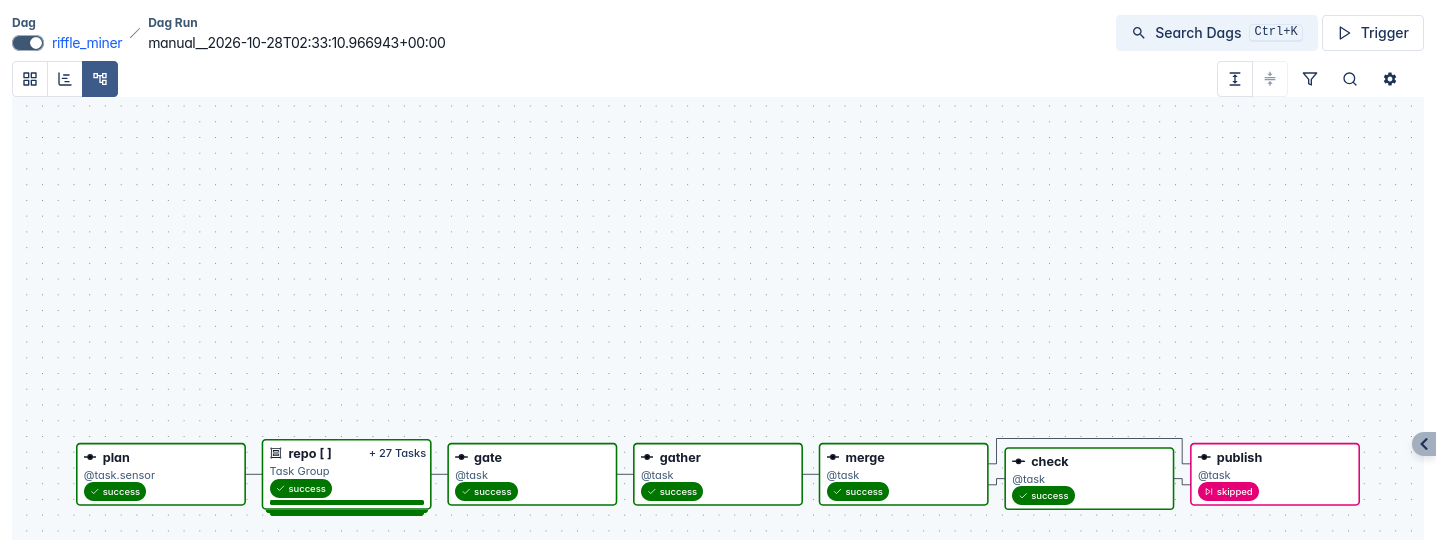
\includegraphics[width=\textwidth]{figures/dag_graph.png}
\caption{Graph view of the \code{riffle_miner} run. The \code{repo} task group holds 27 tasks per repository (collapsed here). \code{publish} is skipped because no DVC remote was given.}
\label{fig:dag}
\end{figure}

\begin{figure}[!htbp]
\centering
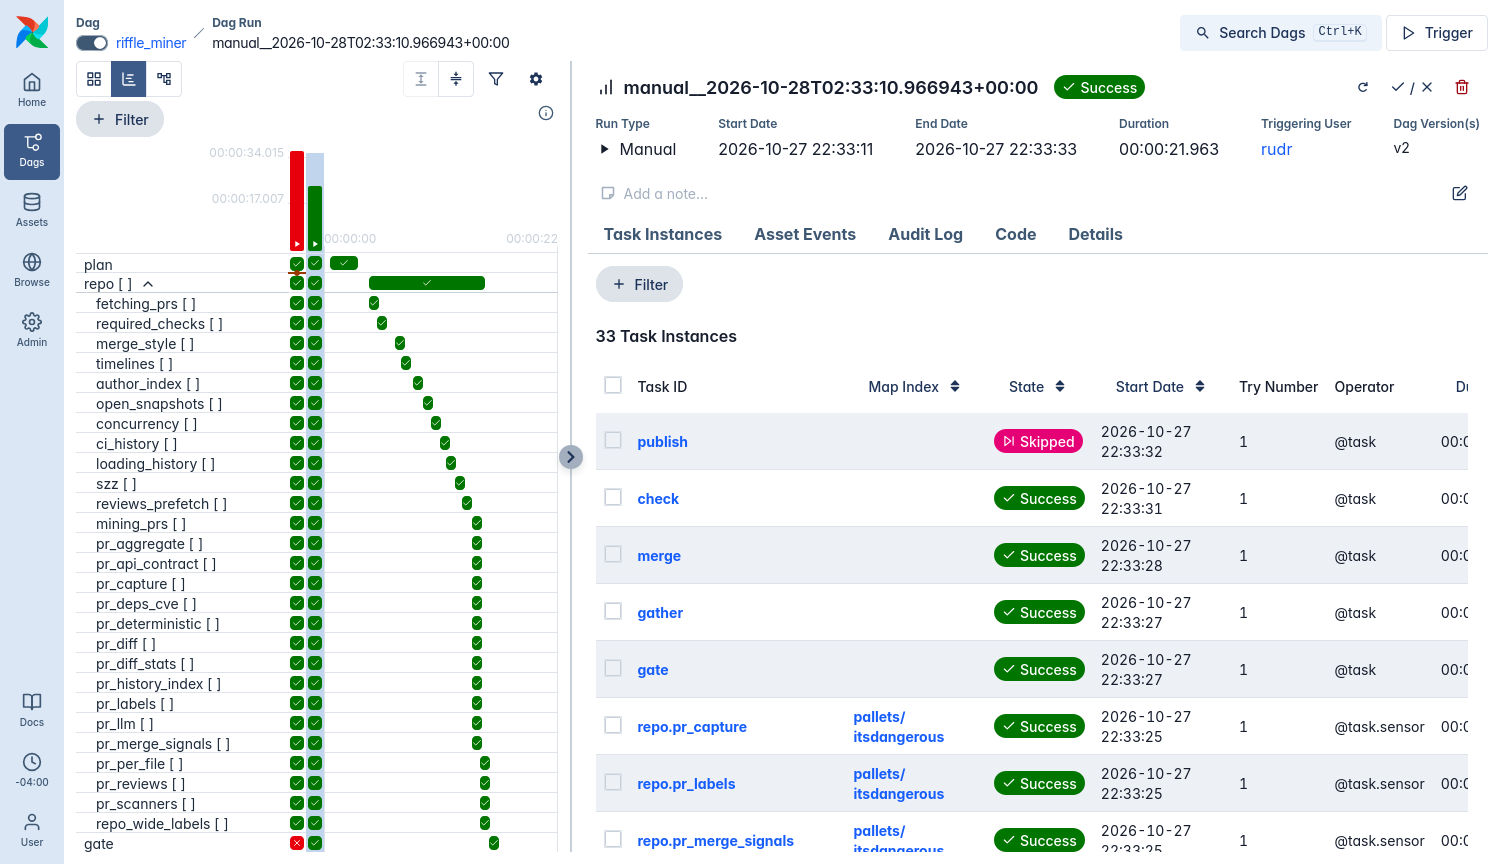
\includegraphics[width=\textwidth]{figures/dag_gantt.png}
\caption{Gantt view of the same run. The per-repository stages (\texttt{fetching\_prs} to \texttt{reviews\_prefetch}) run one after another; the \texttt{pr\_*} steps and \texttt{mining\_prs} then run side by side, followed by \texttt{gate}.}
\label{fig:gantt}
\end{figure}

\begin{figure}[!htbp]
\centering
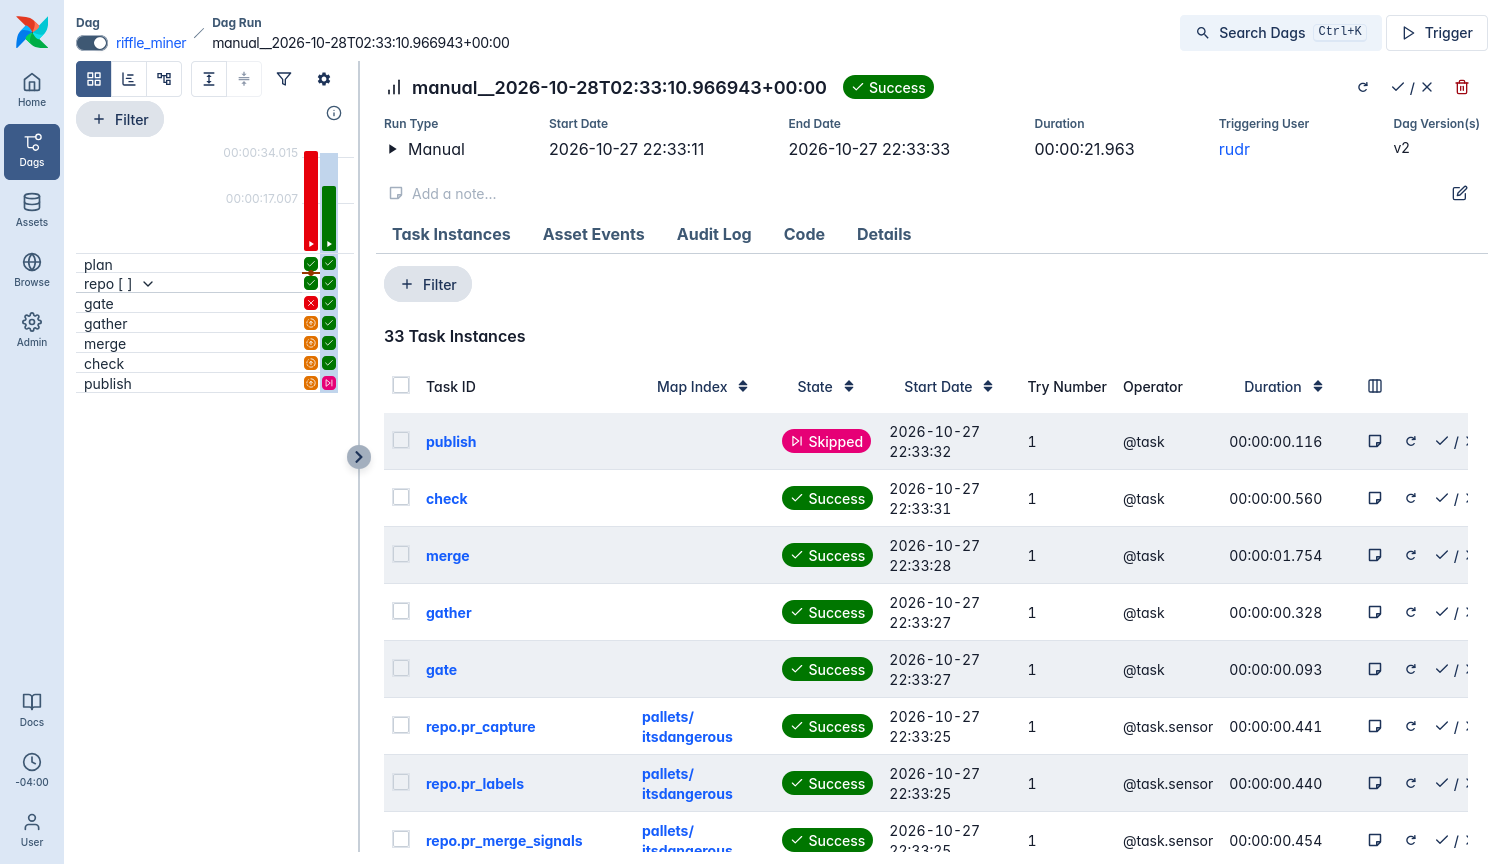
\includegraphics[width=\textwidth]{figures/dag_run_tasks.png}
\caption{The run succeeded in 21.96 seconds with 33 task instances. \code{merge} took 1.75 s, \code{check} 0.56 s and \code{gather} 0.33 s.}
\label{fig:tasks}
\end{figure}

\begin{figure}[!htbp]
\centering
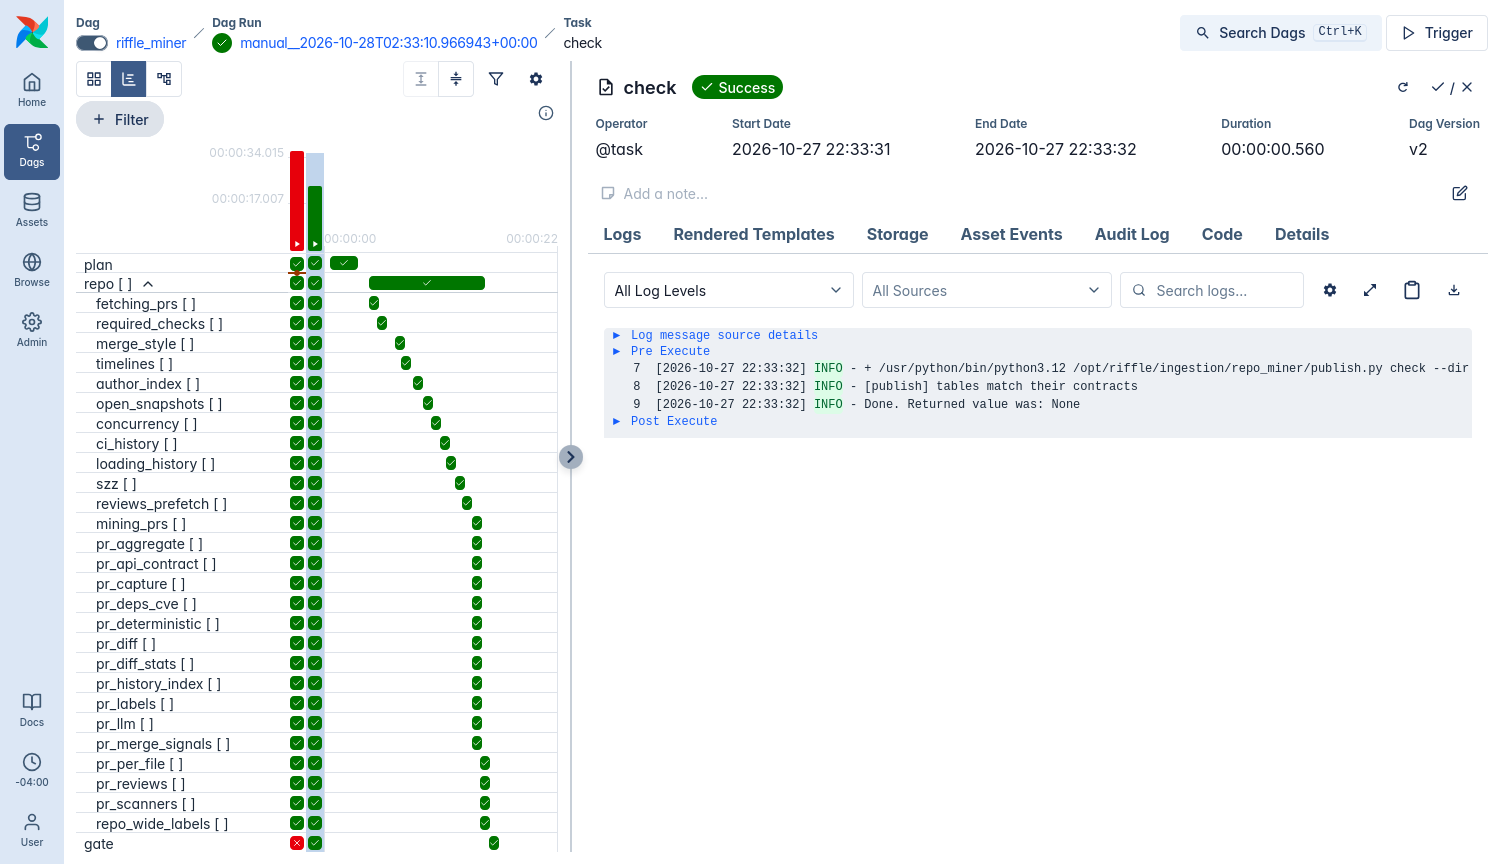
\includegraphics[width=\textwidth]{figures/dag_log_check.png}
\caption{Log of the \code{check} task: the merged tables match their contracts.}
\label{fig:checklog}
\end{figure}

\textbf{Reading the Gantt chart (flow optimisation).} In this demo the slowest real task is \code{merge} (1.75 s). The \code{check} and \code{gather} tasks are short. The stage chain in front of mining is serial by design, because each stage reads the previous stage's trace, and the 14 \texttt{pr\_*} steps already run in parallel with \texttt{mining\_prs}. On a real run the time is spent by the miner on the PCs, not in Airflow: the stage tasks are sensors that poll the store's traces every 30 seconds in \texttt{reschedule} mode, so they hold no worker while they wait. Parallelism is capped at 12 tasks (\texttt{AIRFLOW\_\_CORE\_\_PARALLELISM}) to keep a small VM from running out of memory. A demo this small cannot show a real bottleneck, so a Gantt chart of a full multi-repository run is still needed to name one.

\subsection{Data versioning with DVC}\label{sec:dvc}
I copied the merged tables the DAG wrote and ran the same \code{publish.py} commands the DAG uses, with a local folder as the DVC remote.

\begin{figure}[!htbp]
\centering
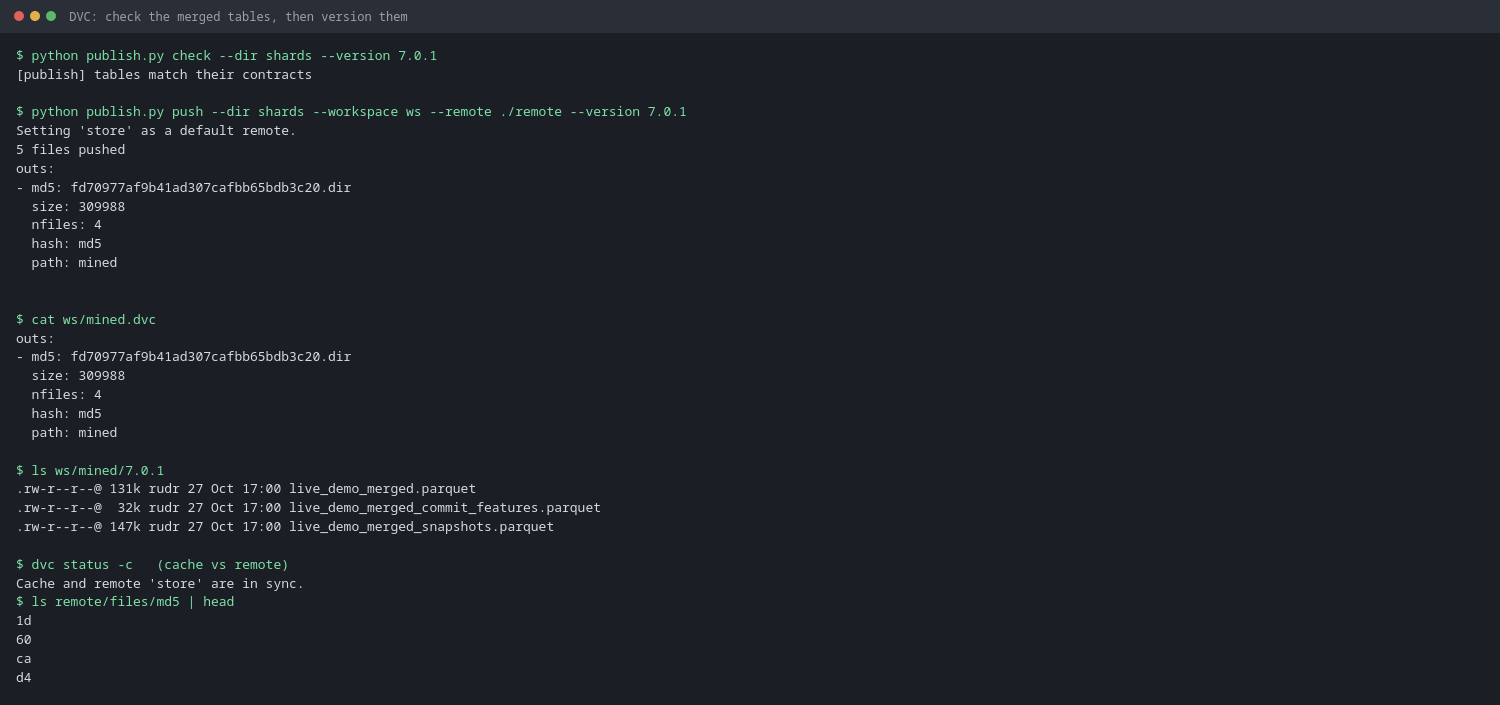
\includegraphics[width=\textwidth]{figures/dvc_run.png}
\caption{\code{publish.py check} passes, then \code{publish.py push} adds the three merged tables (and their manifest) to DVC and pushes them. The pointer \texttt{mined.dvc} holds the content hash; \texttt{dvc status -c} shows cache and remote in sync.}
\label{fig:dvc}
\end{figure}

\subsection{Tests and the slice report}
\begin{figure}[!htbp]
\centering
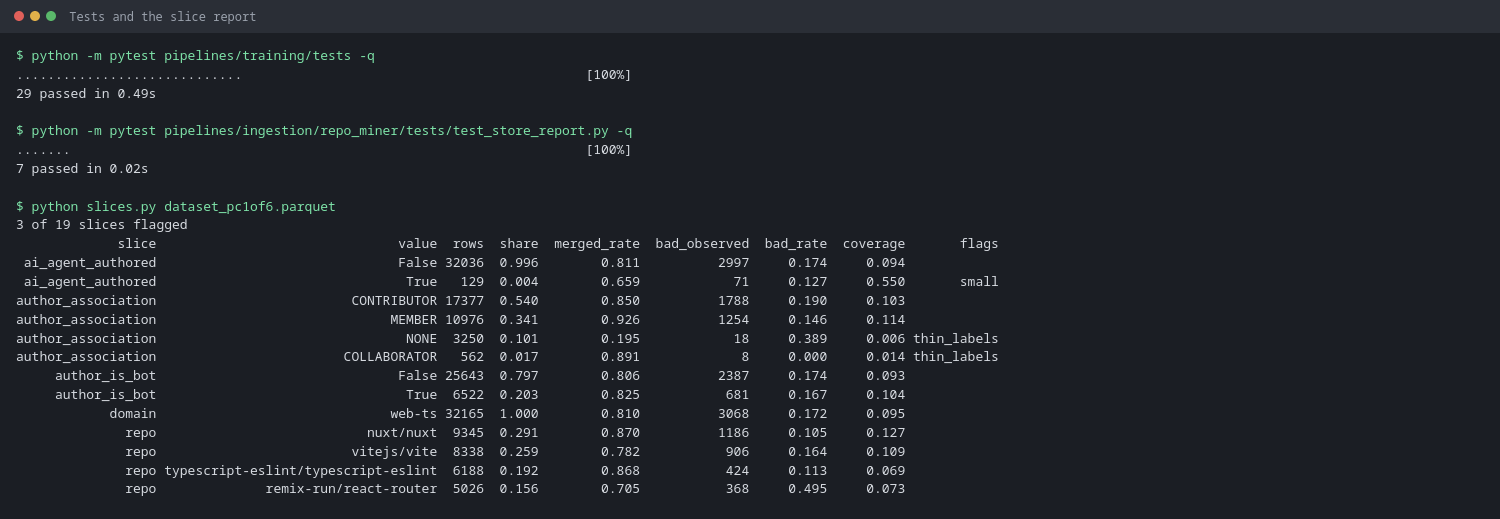
\includegraphics[width=\textwidth]{figures/tests_run.png}
\caption{Unit tests pass (29 in the training suite, 7 for the store report), and \code{slices.py} flags 3 of 19 slices on the real shard.}
\label{fig:tests}
\end{figure}

\subsection{Team store}
\begin{figure}[!htbp]
\centering
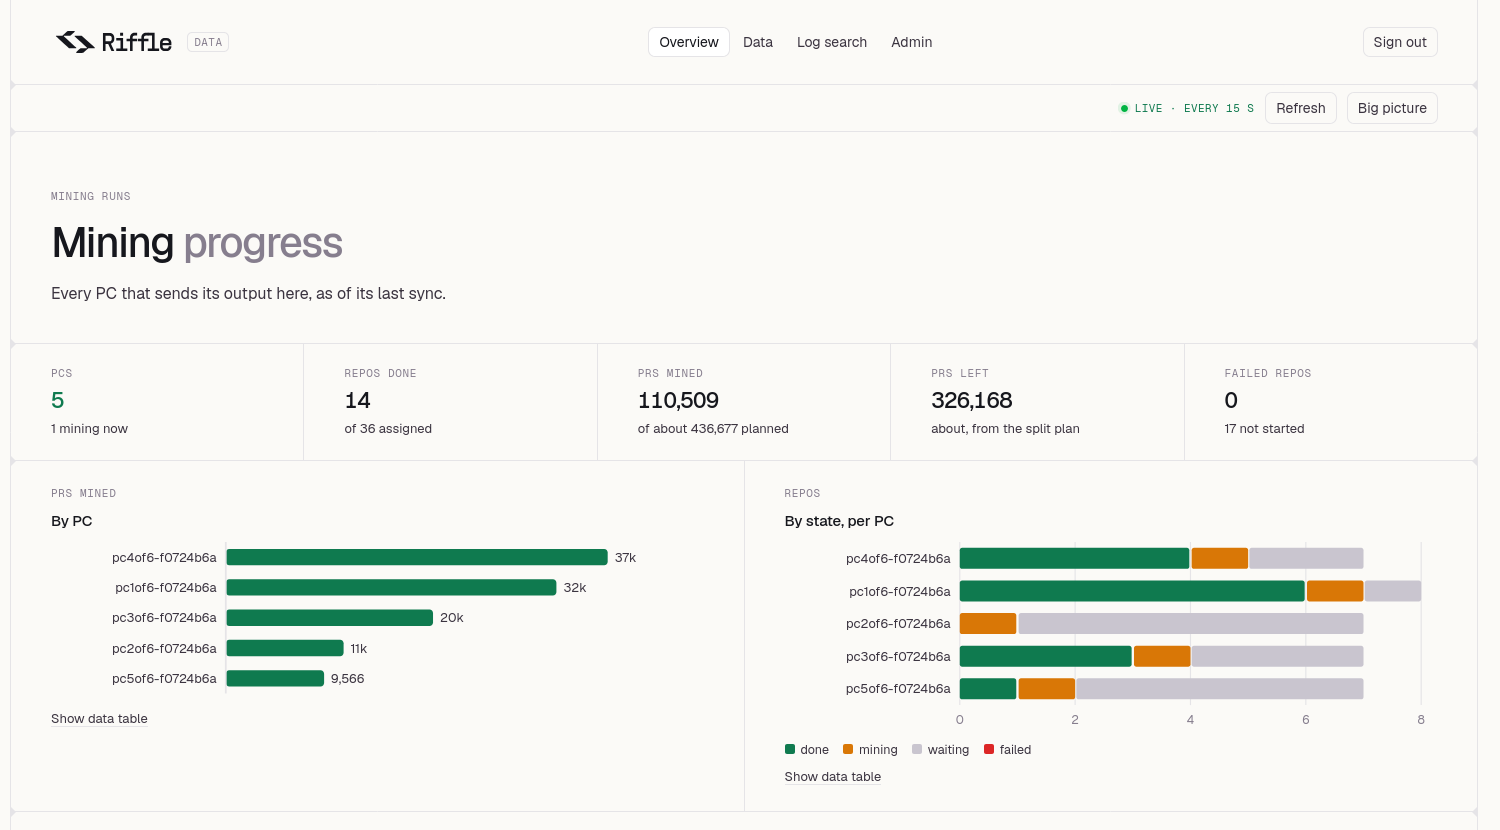
\includegraphics[width=\textwidth]{figures/store_overview.png}
\caption{The team store's overview page: five PCs, 14 of 36 repositories done, 110,509 PRs mined of about 436,677 planned at the time of capture. The store's page covers the five PCs that had uploaded; section~\ref{sec:store} adds PC 6.}
\label{fig:store_page}
\end{figure}

%--------------------------------------------------------------------
\section{Dashboards and Monitoring}\label{sec:dash}

The miner is monitored from three places: a terminal UI on each PC, a read-only web view of that UI, and the team store's pages. All three read the same run events and traces, so they agree. This section shows each one from a real run.

\textbf{The run.} I started the miner's own \emph{Test run} in the TUI on 27 October 2026. It mined 10 closed PRs from \texttt{pallets/flask}: 10 rows with 210 columns in 10 to 16 seconds. LLM flags were off, so no Claude quota was used, and the team-store upload was switched off so nothing from this test reached the team store. The first run needed no clone work because the repository was already cached.

\subsection{Terminal UI}
\code{tui.py} is where a PC starts and watches a run. The left side is the configuration form (repos file, shard K of N, workers, LLM and SZZ switches). The right side shows overall progress, a table per repository (stage, PRs, SZZ, rows, skips, LLM ok and fail, time, ETA, slowest PR) and the live log. It also joins a team store, issues join codes for the lead, and checks the environment first with \code{doctor.py}.

\begin{figure}[!htbp]
\centering
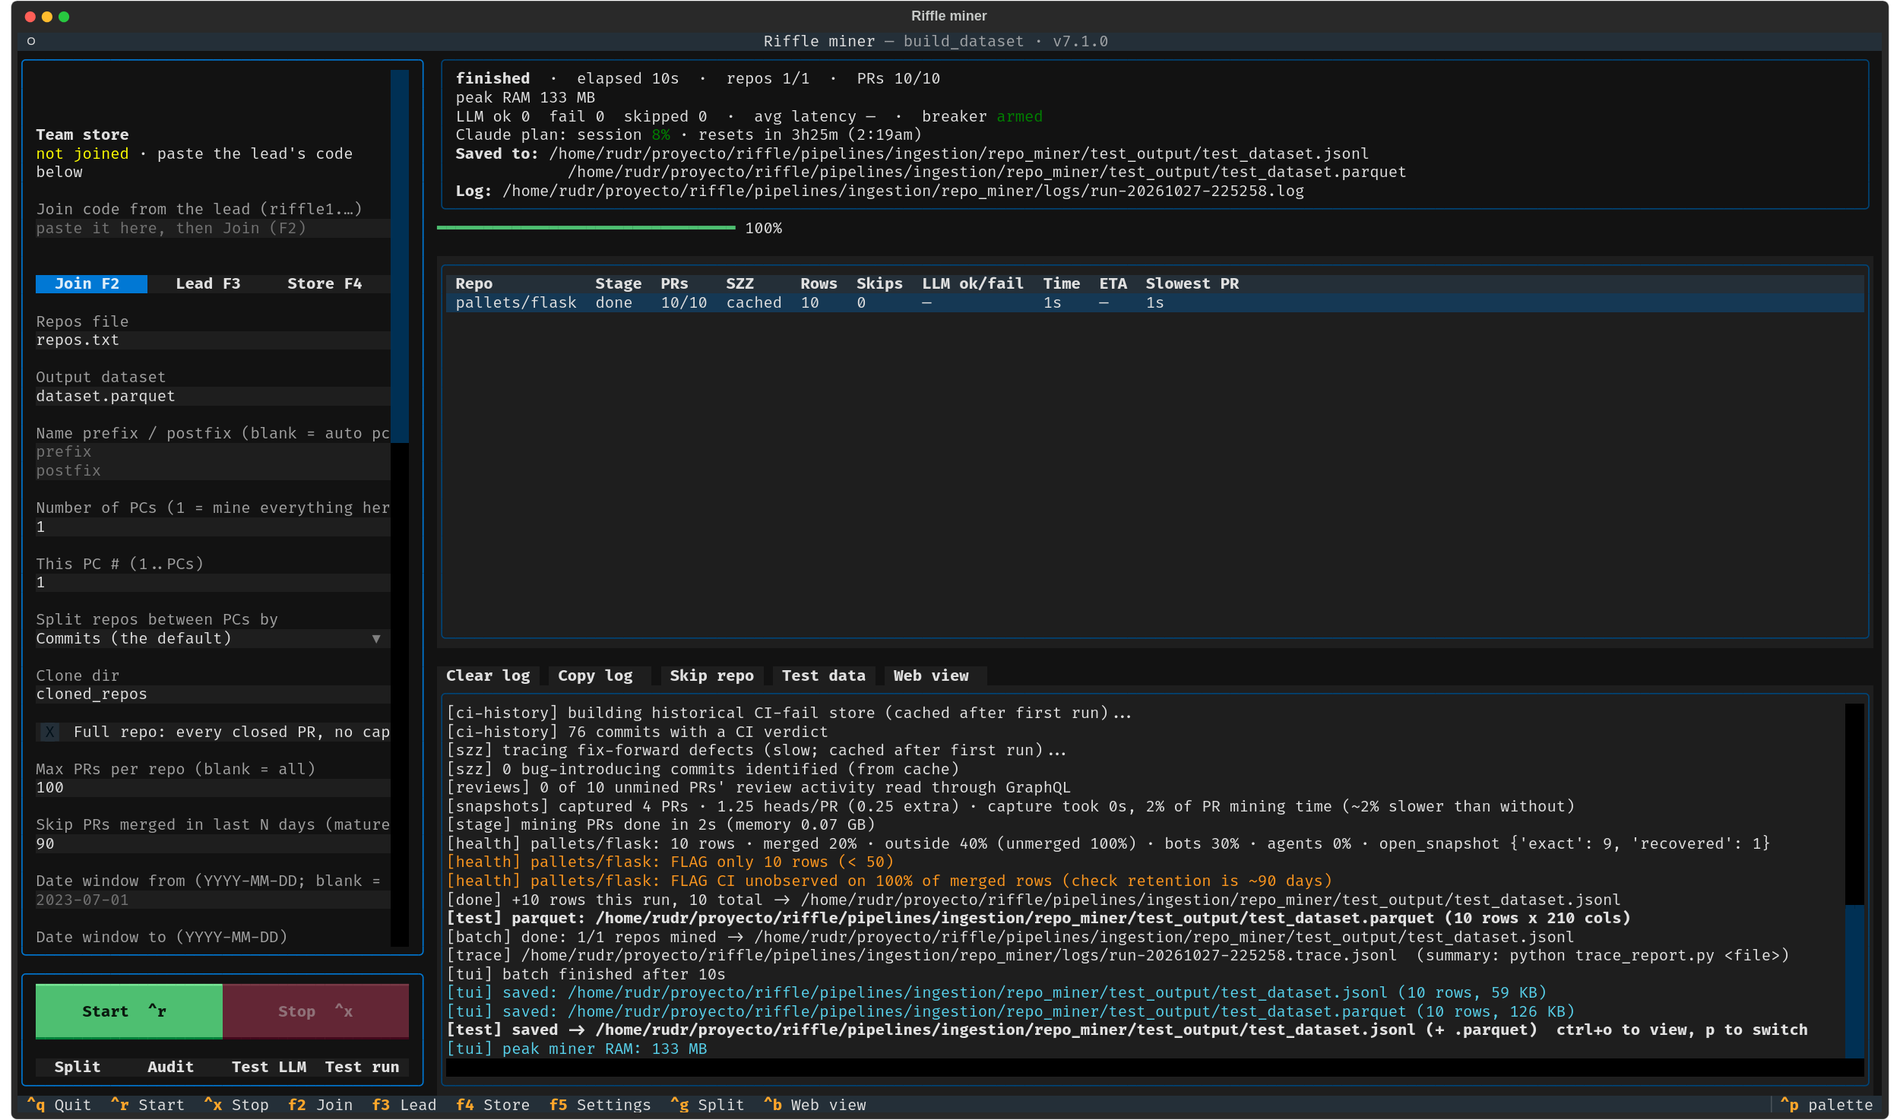
\includegraphics[width=\textwidth]{figures/tui_main.png}
\caption{The TUI after the test run: 100\% of 10 PRs, one repository row, and the log with the health flags. Left: the run form and the team-store card.}
\label{fig:tuimain}
\end{figure}

The \emph{Test data} button opens the mined rows in place, so a run can be checked before it is trusted.

\begin{figure}[!htbp]
\centering
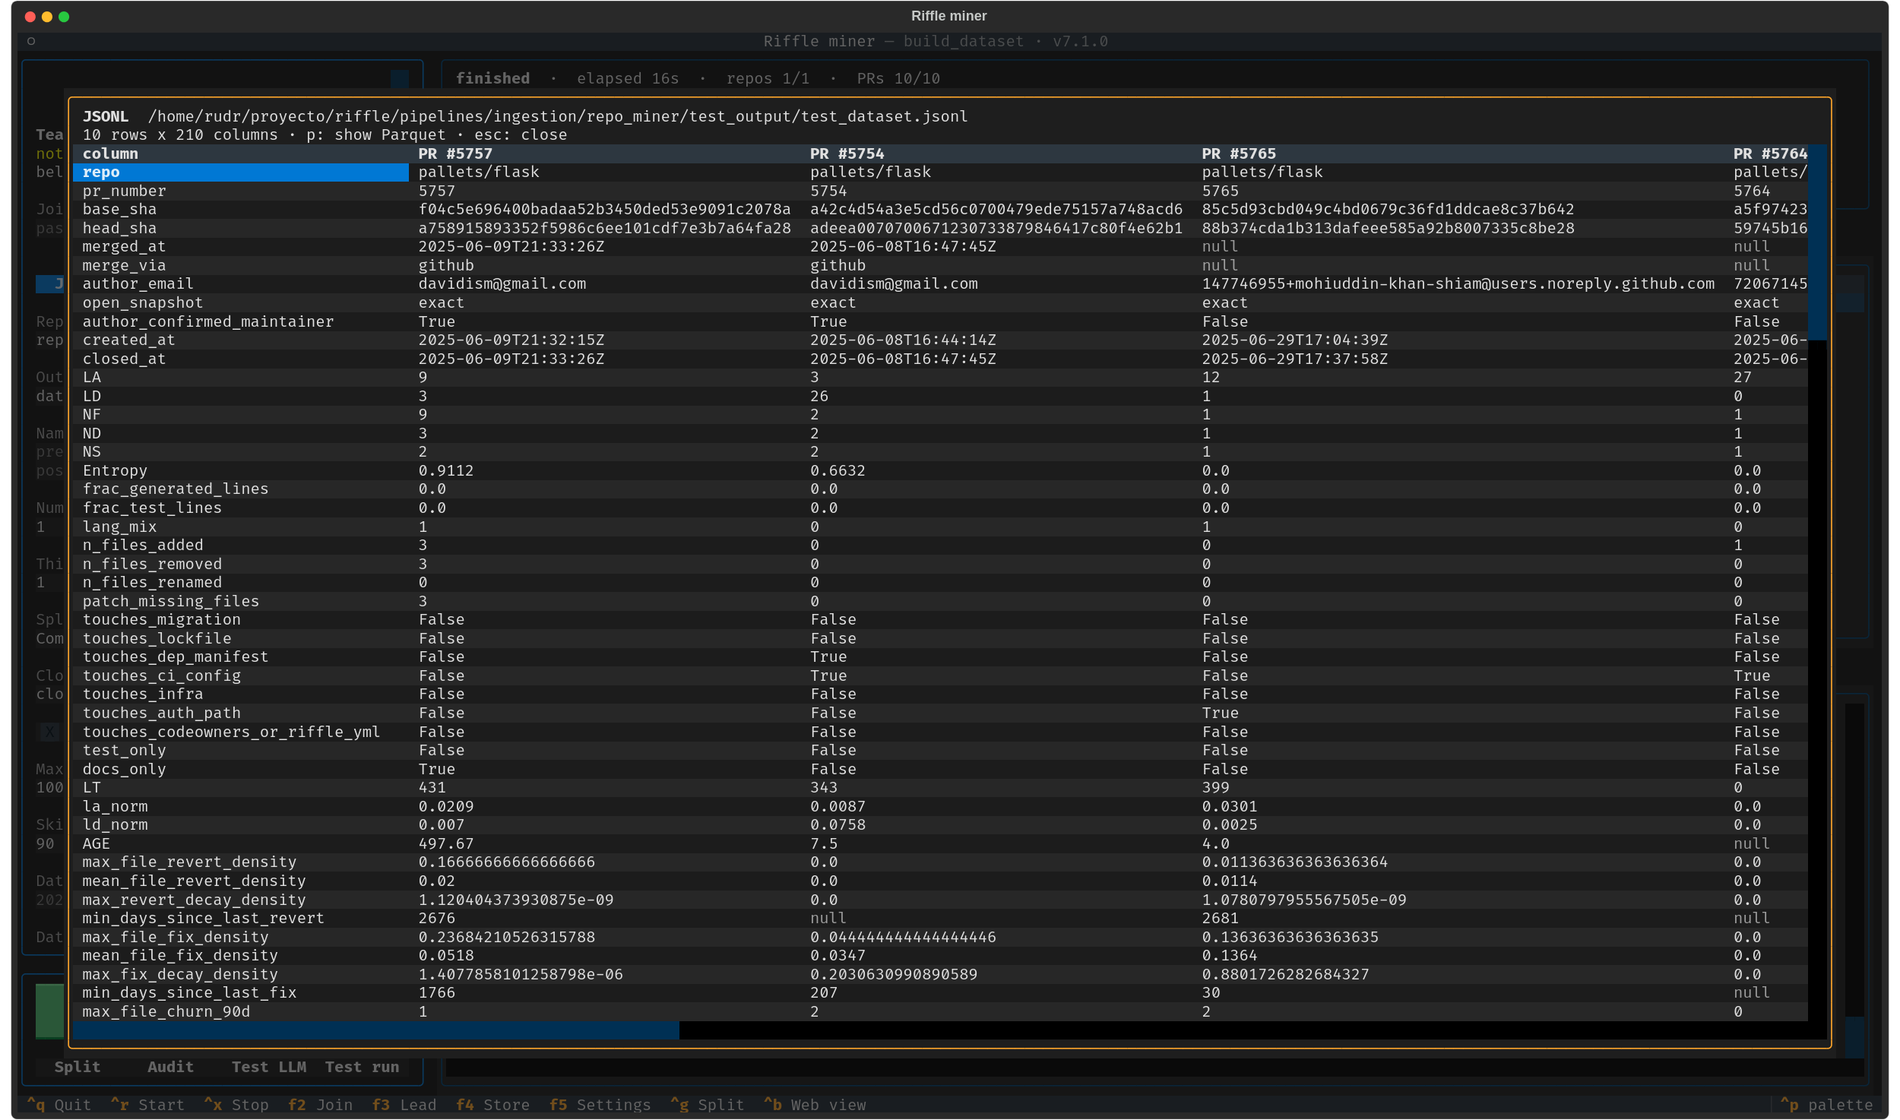
\includegraphics[width=\textwidth]{figures/tui_data_viewer.png}
\caption{The TUI's data viewer on the test run: 10 rows by 210 columns, one column per feature or label, one column of values per PR.}
\label{fig:tuiviewer}
\end{figure}

\subsection{Local web view and big picture}
The TUI also serves a read-only web view on the local network, behind a random key that changes at each launch. A phone or second screen can follow the run without touching it. It shows the same numbers as the TUI plus memory, CPU, the Claude plan's session use and a searchable log. The \emph{big picture} is one full-screen view for a screen across the room.

\begin{figure}[!htbp]
\centering
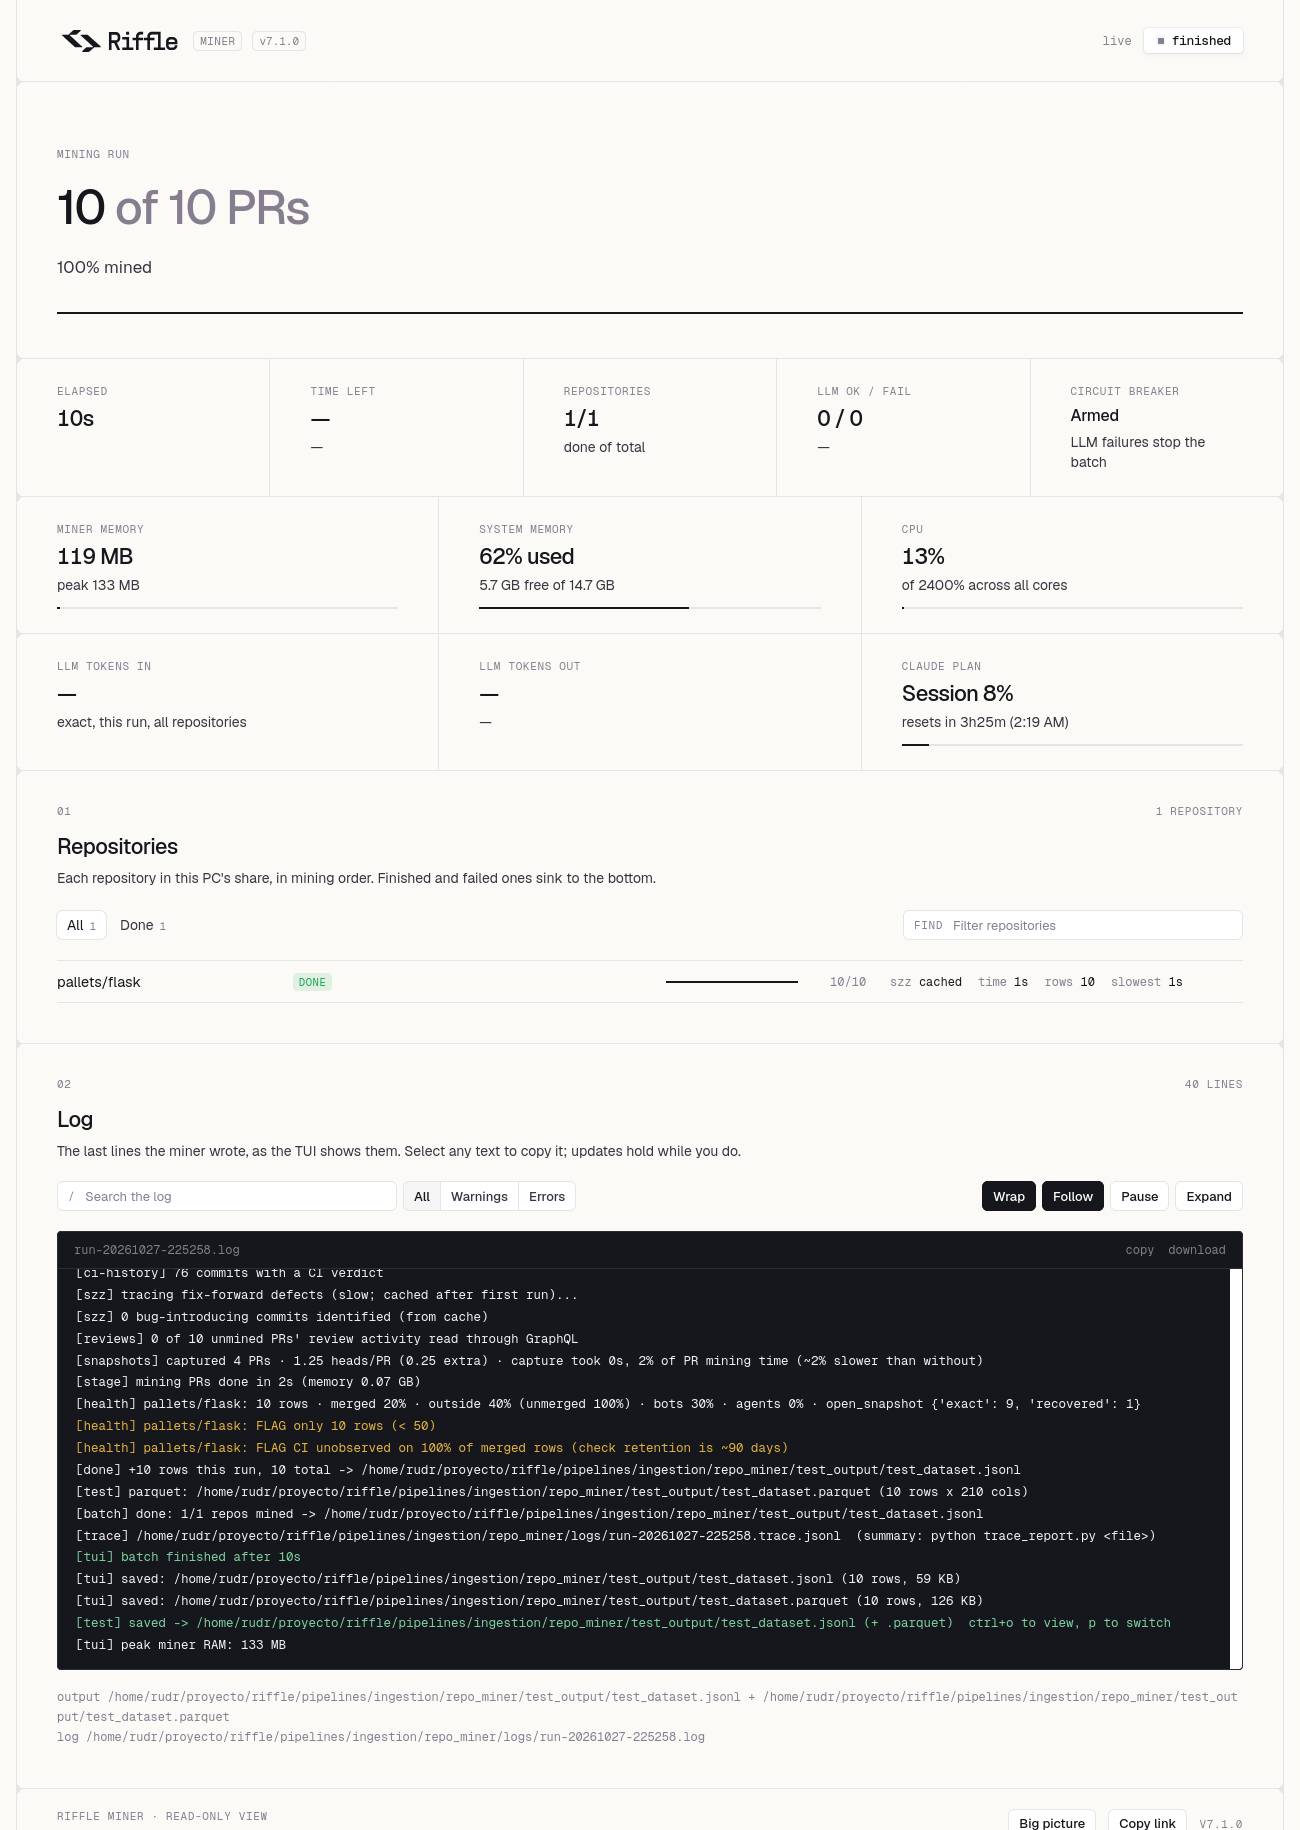
\includegraphics[width=0.78\textwidth]{figures/miner_web_view.png}
\caption{The local web view after the test run: progress, time left, repositories, LLM ok and fail, circuit breaker, memory and CPU, the repository list and the log with its warnings.}
\label{fig:webview}
\end{figure}

\begin{figure}[!htbp]
\centering
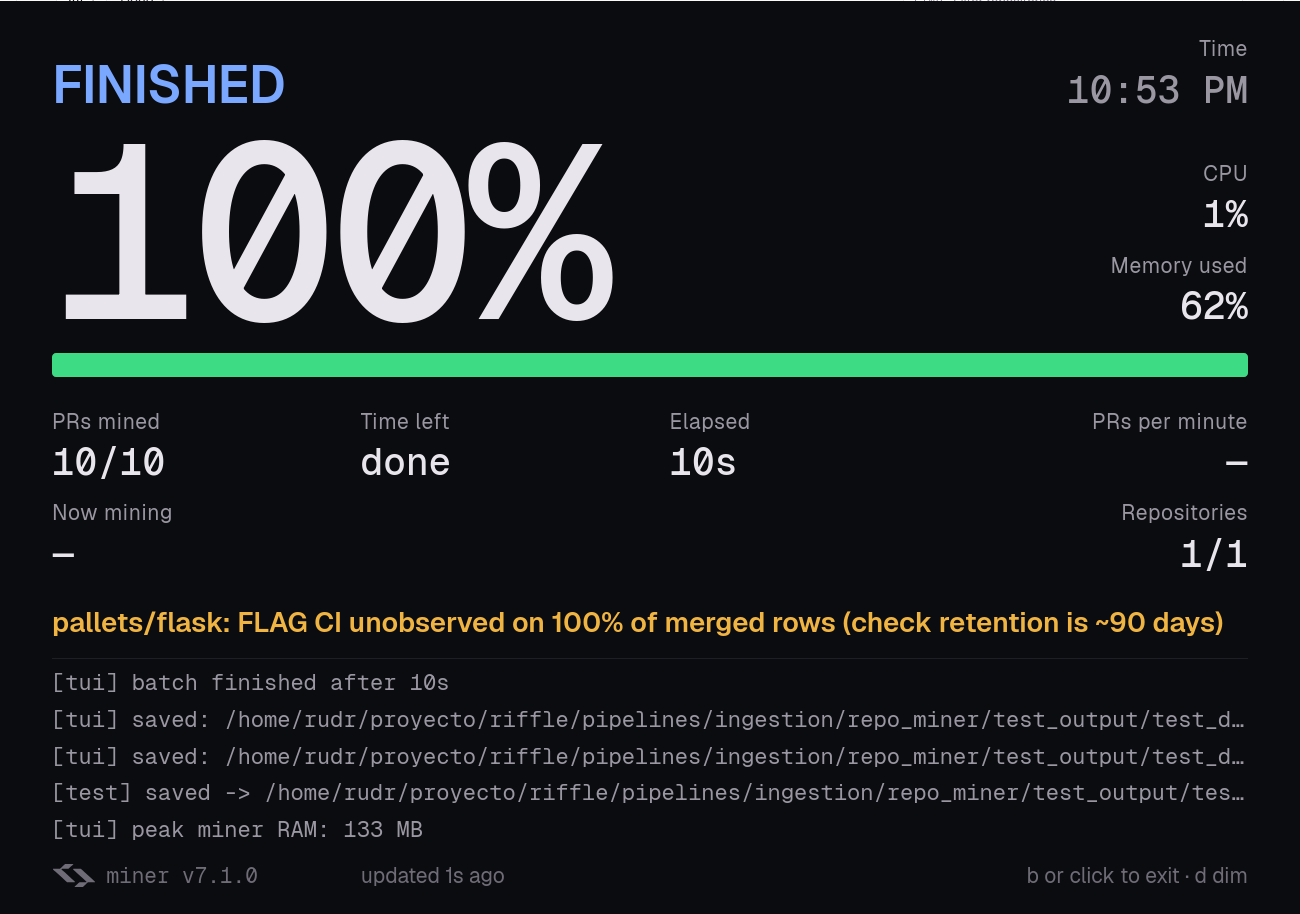
\includegraphics[width=0.75\textwidth]{figures/miner_big_picture.png}
\caption{The local big picture: progress, PRs mined, time left, CPU and memory, and the latest health warning (CI labels unobserved on all merged rows of this tiny sample).}
\label{fig:minerbig}
\end{figure}

\subsection{Team store: progress of all PCs}
Each PC sends its run to the team store on the GCP VM. The store shows every PC on one page (Figure~\ref{fig:store_page}) and, like the miner, has a big picture for a wall screen (Figure~\ref{fig:storebig}).

\begin{figure}[!htbp]
\centering
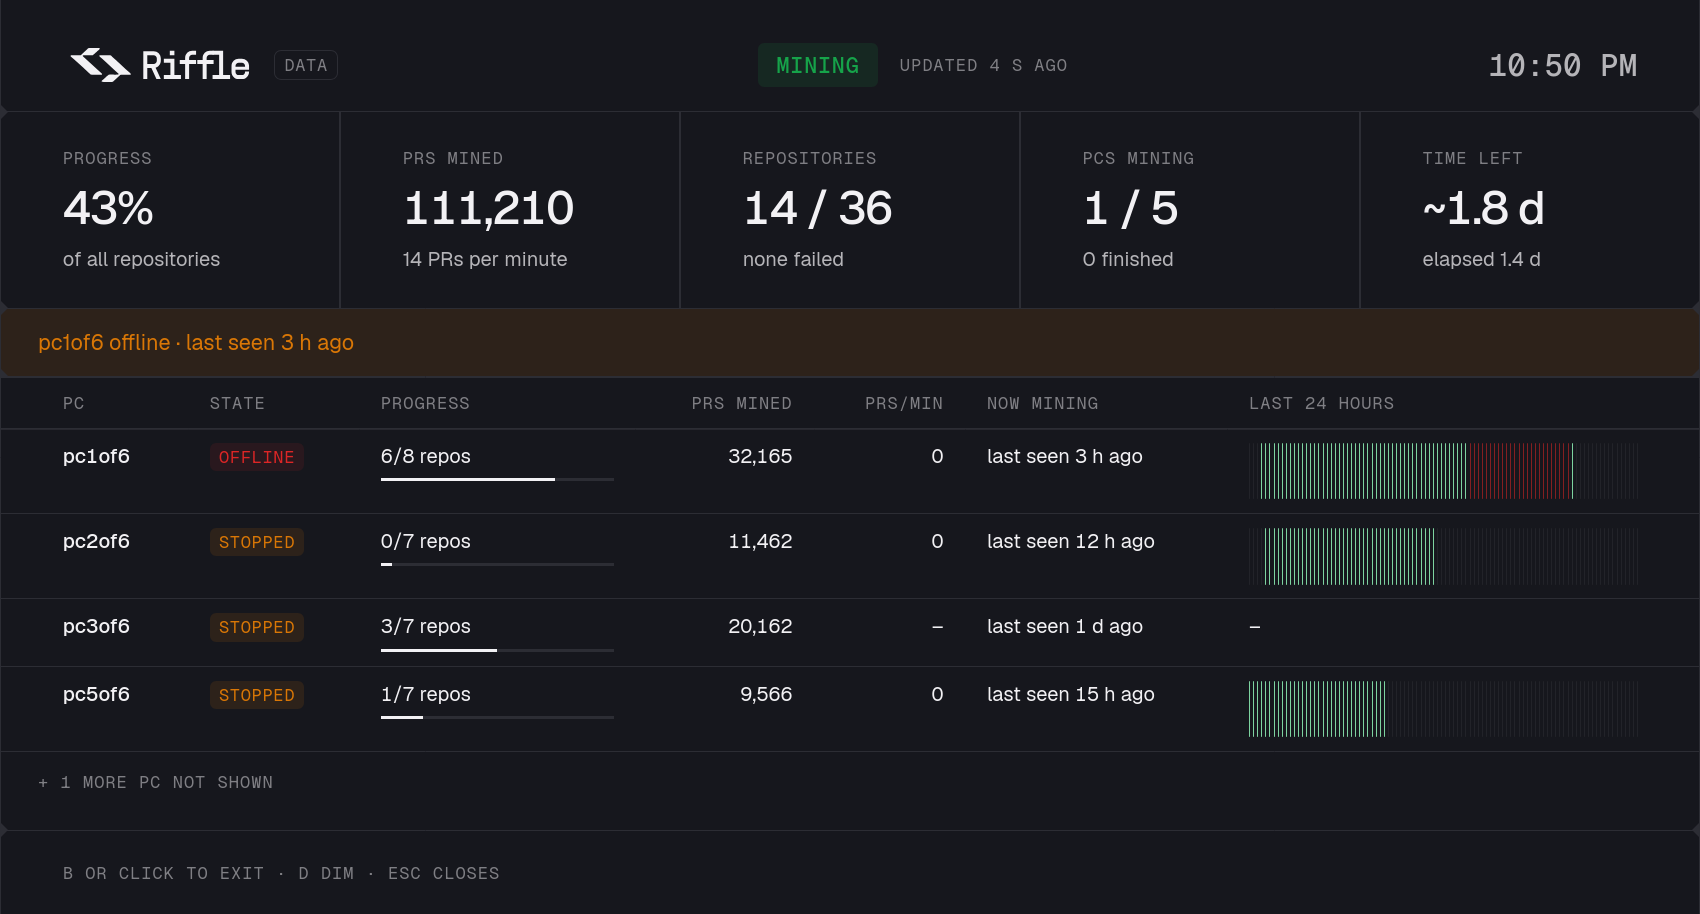
\includegraphics[width=\textwidth]{figures/store_big_picture.png}
\caption{The store's big picture of the real mining run: 43\% of all repositories, 111,210 PRs mined at 14 PRs per minute, about 1.8 days left, and an \emph{offline} banner for PC 1, which had stopped syncing three hours earlier. The activity strip shows each PC's last 24 hours.}
\label{fig:storebig}
\end{figure}

The store's time-left figure is a projection from the recent PRs-per-minute rate. The counts in section~\ref{sec:store} are PRs planned, mined and pending. Both say mining needs days, not hours, because 524,413 PRs are planned across the six PCs.

\subsection{What the dashboards monitor}
\begin{itemize}
  \item \textbf{Progress and speed:} PRs mined, PRs per minute, time left, repository state per PC.
  \item \textbf{Health of the data:} the \code{health.py} flags appear in the log of all three views as soon as a repository finishes (row count under 50, unobserved CI, bot share, missing LLM columns).
  \item \textbf{Health of the machine:} miner and system memory, CPU, and the circuit breaker that stops a batch when the LLM keeps failing.
  \item \textbf{Health of the team:} a PC that stops syncing turns \emph{offline}, and a stopped run is shown as stopped, never as done.
\end{itemize}

\section[Data Bias Detection Using Data Slicing]{Data Bias Detection Using Data Slicing \hfill \pending}\label{sec:bias}

\subsection{Tool}
\code{pipelines/training/slices.py} is new in this draft. It reads the dataset table and reports label balance per slice, so groups the model would learn badly show up before training.

\begin{verbatim}
python pipelines/training/slices.py dataset_merged.parquet \
    --out slices.csv [--strict]
\end{verbatim}

Per slice value it gives: rows, share, merged rate, number of rows with an observed \code{label_bad}, the bad rate over those rows only, and label coverage. It flags a slice as \texttt{small} (under 200 rows) or \texttt{thin\_labels} (under 50 observed rows). An unobserved label is never counted as ``not bad'': the bad rate is null when nothing is observed. \texttt{--strict} exits 1 when any slice is flagged, so it can gate a DAG task. Slice columns and thresholds are arguments, not repository rules. Seven pytest cases cover rates, null handling, flags, missing columns, empty input and the exit codes; the training suite passes (29 tests).

\subsection{Data and method}
The run used the miner shard \code{dataset_pc1of6.parquet}: 32,165 closed PRs from 6 repositories, created May 2014 to August 2026, miner versions 6.12.1 to 7.0.1, one domain tag (\code{web-ts}). Only 3,068 rows (9.5\%) have an observed \code{label_bad}, because the label needs a closed observation window after merge. The numbers are indicative: one shard, mixed miner versions.

\subsection{Findings}

\begin{center}
\small
\begin{tabular}{@{}lrrrrr@{}}
\toprule
\code{author_association} & Rows & Merged & Observed & Bad rate & Flag \\
\midrule
CONTRIBUTOR & 17,377 & 0.850 & 1,788 & 0.190 & \\
MEMBER & 10,976 & 0.926 & 1,254 & 0.146 & \\
NONE & 3,250 & 0.195 & 18 & 0.389 & thin\_labels \\
COLLABORATOR & 562 & 0.891 & 8 & 0.000 & thin\_labels \\
\midrule
\code{ai_agent_authored} = true & 129 & 0.659 & 71 & 0.127 & small \\
\code{ai_agent_authored} = false & 32,036 & 0.811 & 2,997 & 0.174 & \\
\code{author_is_bot} = true & 6,522 & 0.825 & 681 & 0.167 & \\
\code{author_is_bot} = false & 25,643 & 0.806 & 2,387 & 0.174 & \\
\bottomrule
\end{tabular}
\end{center}

\begin{center}
\small
\begin{tabular}{@{}lrrrr@{}}
\toprule
Repository & Rows & Merged & Observed & Bad rate \\
\midrule
nuxt/nuxt & 9,345 & 0.870 & 1,186 & 0.105 \\
vitejs/vite & 8,338 & 0.782 & 906 & 0.164 \\
typescript-eslint/typescript-eslint & 6,188 & 0.868 & 424 & 0.113 \\
remix-run/react-router & 5,026 & 0.705 & 368 & \textbf{0.495} \\
preactjs/preact & 2,687 & 0.765 & 130 & 0.069 \\
solidjs/solid & 581 & 0.764 & 54 & 0.296 \\
\bottomrule
\end{tabular}
\end{center}

\begin{center}
\small
\begin{tabular}{@{}lrrrr@{}}
\toprule
PR size quartile (LA + LD) & Rows & Merged & Observed & Bad rate \\
\midrule
Q1 (smallest) & 8,071 & 0.793 & 597 & 0.127 \\
Q2 & 8,026 & 0.831 & 671 & 0.161 \\
Q3 & 8,037 & 0.808 & 796 & 0.173 \\
Q4 (largest) & 8,031 & 0.810 & 1,004 & 0.206 \\
\bottomrule
\end{tabular}
\end{center}

\begin{enumerate}
  \item \textbf{Outside contributors have almost no breakage labels.} \texttt{NONE} PRs (authors with no prior link to the repository) merge 19.5\% of the time against 85 to 93\% for the rest, so most of them never reach the post-merge label. Only 18 of 3,250 rows (0.6\%) are observed, so the 38.9\% bad rate rests on 18 examples. A breakage model trained on this table has effectively no signal on this group.
  \item \textbf{The repositories differ more than the author groups do.} The bad rate is 49.5\% in react-router against 7 to 16\% in four others, and the merged rate ranges from 0.705 to 0.870. A model can learn repository habits as risk. The two largest repositories hold 55\% of rows.
  \item \textbf{AI-agent PRs are 0.4\% of rows.} The 129 rows are too few to learn from, although 55\% of them have an observed label.
  \item \textbf{Size is a real signal, not a bias.} The bad rate rises from 12.7\% to 20.6\% across size quartiles.
  \item \textbf{Single domain.} Every row is \code{web-ts}, so no cross-domain slice exists in this shard.
  \item Collaborator's 0.000 bad rate rests on 8 observed rows and means nothing.
\end{enumerate}

\subsection{Mitigation plan (not yet applied)}
Training is not built, so no mitigation has been run and no before/after number exists. The plan:

\begin{center}
\small
\begin{tabular}{@{}p{4.2cm}p{5.6cm}p{4.6cm}@{}}
\toprule
Problem & Technique & Trade-off \\
\midrule
\texttt{NONE} slice has 18 labels & Report per-slice metrics; keep \code{label_bad_observed} as a mask; use the merge-outcome frame (snapshots, which covers unmerged PRs) for this group & Breakage claims for this group stay unproven \\
Agent slice too small & Mine more agent-authored PRs with our own miner, using the detector tested on AIDev; report this slice separately & Slower; the agent share of new PRs sets the pace \\
Repository skew & Cap rows per repository, or hold out by repository (\code{by="repo"} already exists in \code{frames.py}) & Loses data from large repositories; a held-out repository measures generalisation honestly \\
Thin outsider class & Collapse to three classes if a slice stays under about 200 examples (data-management plan) & Less detail in the label \\
Reporting & Per-slice metric table each training run (Fairlearn \texttt{MetricFrame} or TFMA) & One more step in training \\
\bottomrule
\end{tabular}
\end{center}

Success check: per-slice recall for \texttt{NONE}, \texttt{CONTRIBUTOR}, \texttt{MEMBER} and agent PRs within an agreed gap (for example 0.05), reported together with the change in the overall metric.

\section{Team Store and Live Progress}\label{sec:store}

The miner runs on six machines. Each one sends its logs, health files, tables and a \code{run.json} to a team store on a Google Cloud VM (ADR 0015). The store keeps the tables in a bucket, queries them with DuckDB, and serves pages that show progress per machine, charts of each table, and searchable logs.

\subsection{Read access for the teaching assistant}
The store is read-only for this token. It can view the pages and the JSON API, and it cannot write, issue tokens or change anything.

\begin{center}
\begin{tabular}{@{}ll@{}}
\toprule
Site & \texttt{https://34-72-217-36.sslip.io/login} \\
Sign-in & paste the read token below into the sign-in box \\
\bottomrule
\end{tabular}
\end{center}

\begin{verbatim}
<read token given to the teaching assistant with the submission>
\end{verbatim}

Pages: \texttt{/} (progress per PC), \texttt{/run} (one PC's run), \texttt{/data} (the three mined tables over every PC), \texttt{/view} (a parquet file as charts and a table) and \texttt{/search} (logs and traces). Scripts can send the token as \texttt{Authorization: Bearer <token>} to \texttt{/api/runs}.

\subsection{Mined and pending, from the admin overview}
The correct counts come from the store's admin overview (\texttt{/v1/admin/overview}), read with the lead's admin token. For every PC token it gives the state (mining, stopped, silent, never), repositories done, repositories in total and PRs mined. It also lists PC 6, which has never uploaded. \code{pipelines/ingestion/repo_miner/store_report.py} reads this overview and the store's run status and draws the charts below. It is read-only, and the admin token is only needed to see the PCs that have not uploaded. The figures are from 28 October 2026.

\textbf{How the numbers are defined.}
\begin{itemize}
  \item \textbf{Planned} is each PC's share of the split plan: the repos file records every PR each repository ever had, and the split gives every PC about 85,000 to 90,000 of them. The six shares add up to 524,413 PRs in 43 repositories.
  \item \textbf{Mined} is the number of rows a PC has written, from the admin overview.
  \item \textbf{Left in the repository being mined} is exact: the PRs the repository selected minus the rows written. Only one repository per PC is in this state.
  \item \textbf{Pending} is planned minus mined. It includes repositories that have not started, whose PRs are not selected yet.
\end{itemize}
The miner keeps the closed PRs inside its window, and finished repositories kept a median of 89\% of their planned PRs. The final total will therefore be somewhat lower than 524,413, and the share mined will be higher than the percentage shown now.

\begin{figure}[!htbp]
\centering
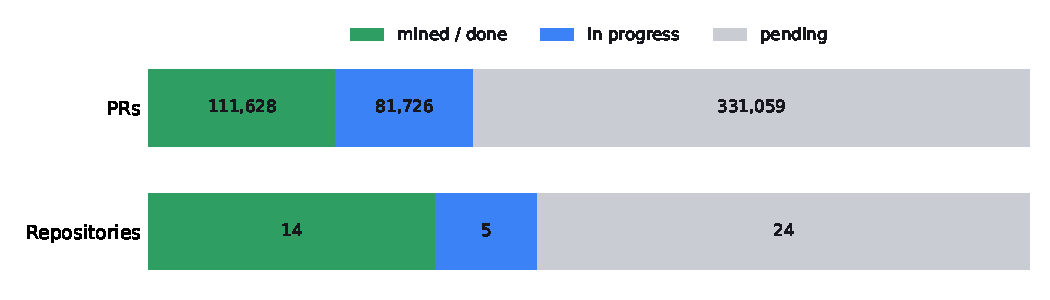
\includegraphics[width=0.95\textwidth]{figures/store_total.pdf}
\caption{Overall progress. PRs: 111,628 mined, 81,726 left in repositories being mined, 331,059 pending, out of 524,413 planned. Repositories: 14 done, 5 in progress, 24 pending, out of 43.}
\label{fig:storetotal}
\end{figure}

\begin{figure}[!htbp]
\centering
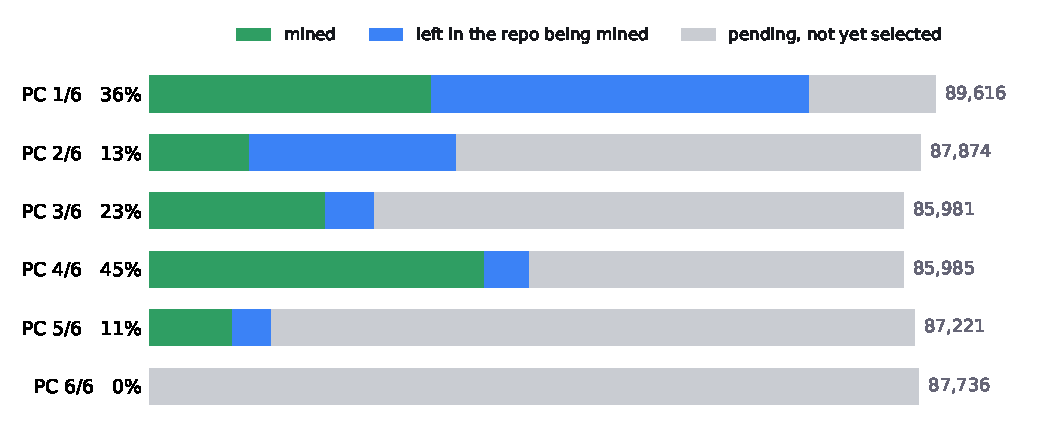
\includegraphics[width=\textwidth]{figures/store_prs.pdf}
\caption{PRs mined and pending per PC, with the share mined at the left of each bar and the planned PRs at the end. PC 6 has never uploaded, so it is fully pending.}
\label{fig:store}
\end{figure}

\begin{figure}[!htbp]
\centering
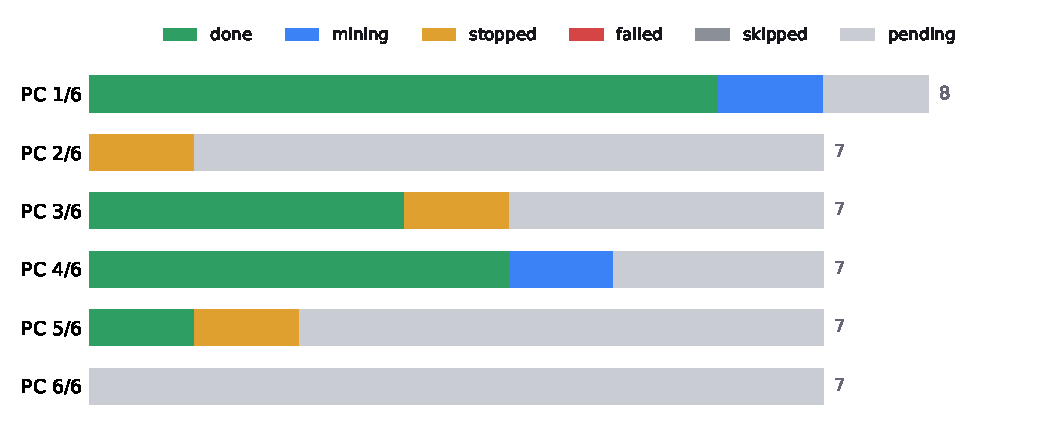
\includegraphics[width=\textwidth]{figures/store_states.pdf}
\caption{Repositories by state per PC. PC 6 has 7 repositories, none started.}
\end{figure}

\begin{figure}[!htbp]
\centering
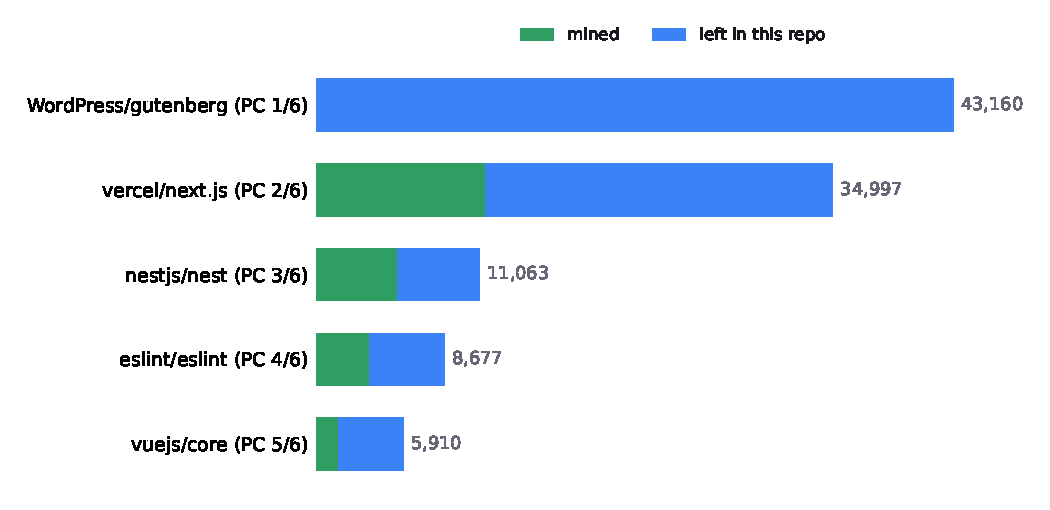
\includegraphics[width=\textwidth]{figures/store_inprogress.pdf}
\caption{The five repositories being mined or stopped part-way, with what is mined and what is left in each (exact).}
\end{figure}

\begin{figure}[!htbp]
\centering
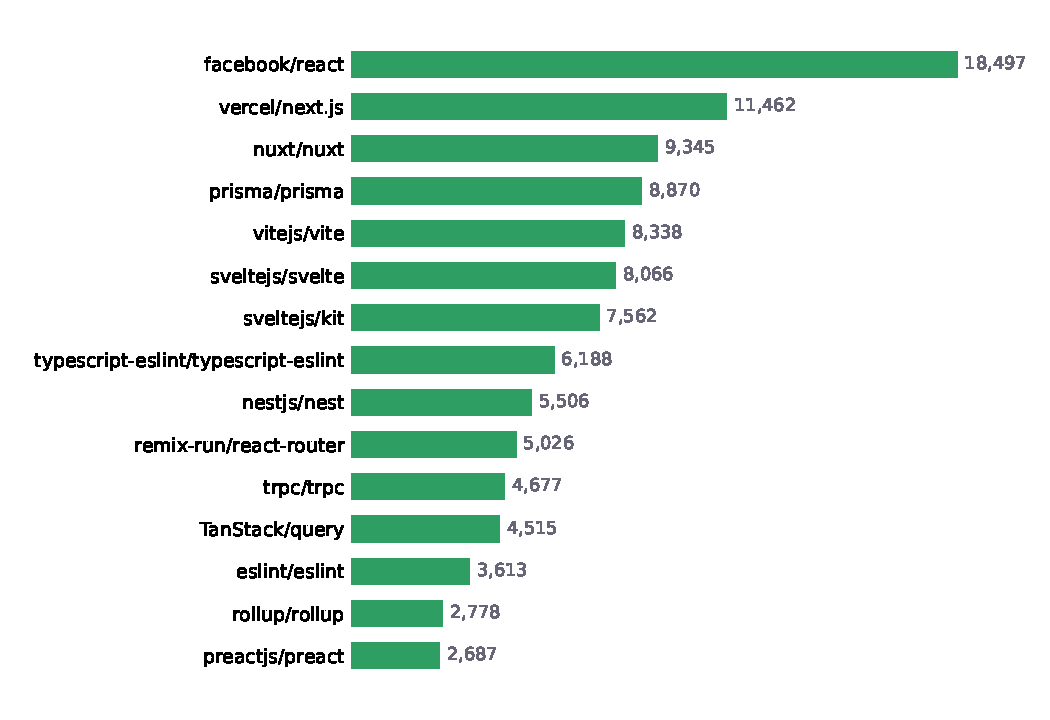
\includegraphics[width=\textwidth]{figures/store_repos.pdf}
\caption{Rows mined per repository across all PCs (top 15).}
\end{figure}

\begin{center}
\small
\begin{tabular}{@{}llrrrr@{}}
\toprule
PC & State & Repos done & Mined & Planned & Mined share \\
\midrule
1 & silent (last upload 27 Oct) & 6 of 8 & 32,165 & 89,616 & 36\% \\
2 & stopped & 0 of 7 & 11,462 & 87,874 & 13\% \\
3 & stopped & 3 of 7 & 20,162 & 85,981 & 23\% \\
4 & mining & 4 of 7 & 38,273 & 85,985 & 45\% \\
5 & stopped & 1 of 7 & 9,566 & 87,221 & 11\% \\
6 & never uploaded & 0 of 7 & 0 & 87,736 & 0\% \\
\midrule
Total & & 14 of 43 & 111,628 & 524,413 & 21.3\% \\
\bottomrule
\end{tabular}
\end{center}

\subsection{Reading the figures}
\begin{itemize}
  \item \textbf{Mined so far: 111,628 PRs}, 21.3\% of the plan, and 14 of 43 repositories done (33\%). The store's own page counts repositories, which is why it shows a higher percentage (Figure~\ref{fig:storebig}).
  \item \textbf{Pending: 412,785 PRs}, of which 81,726 are in repositories already being mined and 331,059 are in repositories not yet selected.
  \item PC 4 is the only PC mining now. PC 1 is silent (its last upload was on 27 October, 22:58 UTC) and PCs 2, 3 and 5 have stopped. PC 6 has not started.
  \item The split is balanced by PR count, so every PC has about the same planned PRs, and the bars end at nearly the same place. The percentages differ because the PCs started at different times and some have stopped.
  \item The bucket behind the store holds 145 files (621 MB), mostly checkpoints (486 MB), which is the data that lets a stopped PC resume.
  \item The machines run different miner versions (7.0.0, 7.0.1, 7.1.0). Tables from different versions must not be merged without checking the contract version, which the \code{check} task of the DAG does against the manifest.
  \item The per-repository chart shows the data is concentrated in the largest repositories. This matters for the bias findings in section~\ref{sec:bias}.
\end{itemize}

%--------------------------------------------------------------------
\section{Additional Guidelines}

\subsection{Folder Structure}
\begin{center}
\small
\begin{tabular}{@{}ll@{}}
\toprule
Guideline & Riffle \\
\midrule
\code{dags/} & \code{pipelines/dags/} \\
\code{scripts/} & \code{pipelines/ingestion/}, \code{infra/docker/airflow/scripts/} \\
\code{tests/} & \code{tests/} beside each package \\
\code{logs/} & \code{logs/} (git-ignored) and Loki \\
\code{data/} & git-ignored, versioned by DVC \\
\code{dvc.yaml} & not present; \code{dvc add} pointers are used \\
\bottomrule
\end{tabular}
\end{center}

\subsection[README Documentation]{README Documentation \hfill \done}
Every directory has a \code{README.md}. \code{repo_miner/README.md} is the operator guide, \code{ARCHITECTURE.md} the full reference, and ADRs in \code{docs/adr/} record each decision. Section~\ref{sec:repro} of this report lists the exact commands to run the pipeline. The root README still describes a target system (\code{make bootstrap}, \code{make up}) that is not built, so a short pointer there is a follow-up.

\subsection[Reproducibility]{Reproducibility \hfill \done}
Pinned dataset revision, miner version in every table, Docker Compose Airflow, Terraform for the store VM and contract-checked outputs. Section~\ref{sec:repro} gives the steps from a fresh clone to a versioned dataset.

\subsection[Code Style]{Code Style \hfill \partialx}
Code is modular, one concern per file. \textbf{Open:} no PEP 8 linter runs in CI yet.

\subsection[Error Handling and Logging]{Error Handling and Logging \hfill \done}
Failure paths are tested: data unavailable, rate limits, force-pushed history, incomplete shards, stale versions and corrupt downloads (hash mismatch in \code{verify.py}). \code{doctor.py} checks the environment before a run, and run traces go to Loki so a failure names its stage, repository and error.

%--------------------------------------------------------------------
\section{Evaluation Criteria Checklist}

\begin{longtable}{@{}rp{3.4cm}p{3.5cm}p{7.3cm}@{}}
\toprule
\# & Criterion & Status & Evidence \\
\midrule
\endhead
1 & Proper documentation & \done & READMEs in every directory, ARCHITECTURE.md, ADRs, this report; reproduction steps in section~\ref{sec:repro} \\
2 & Modular syntax and code & \done & one module per stage \\
3 & Airflow DAG orchestration & \done & \code{riffle_miner.py}, Compose stack \\
4 & Tracking and logging & \done & run traces, Loki, Grafana \\
5 & DVC & \pending & check and push tested (Fig.~\ref{fig:dvc}); the final push of the merged v7 tables comes once the mining target is achieved \\
6 & Flow optimisation & \pending & parallel, sharded, cached; Gantt captured and read (Fig.~\ref{fig:gantt}); full-run Gantt comes once the mining target is achieved \\
7 & Schema and statistics & \done & JSON Schema contracts enforced in CI and before DVC; statistics from \code{health.py} shown in the dashboards \\
8 & Anomalies and alerts & \done & \code{health.py} flags, contract gate, offline banner, Airflow task failures (Figs.~\ref{fig:tuimain}, \ref{fig:webview}, \ref{fig:storebig}); no email/Slack \\
9 & Bias detection and mitigation & \pending & \code{slices.py} built, tested and run on 32,165 PRs; mitigation applies once training exists \\
10 & Test modules & \done & about 60 miner test files, 7 for \code{slices.py} \\
11 & Reproducibility & \done & pins, Docker, Terraform, commands in section~\ref{sec:repro} \\
12 & Error handling and logging & \done & tested failure paths, \code{doctor.py} \\
\bottomrule
\end{longtable}

\section{Reproducing the Pipeline}\label{sec:repro}

These are the commands used for the test run in this report. Run them from the repository root unless a line says otherwise. The mining step needs a GitHub token in \code{pipelines/ingestion/repo_miner/.env}.

\begin{verbatim}
# 1. Python tests (no network, no LLM)
python -m pytest contracts/tests pipelines/ingestion/repo_miner/tests -q
python -m pytest pipelines/training/tests -q

# 2. Mine a small test set with the terminal UI, then press "Test run"
cd pipelines/ingestion/repo_miner && python tui.py
#    or without the UI:
python build_dataset.py --test

# 3. Airflow (Docker Compose), then open http://localhost:8080
cd infra/docker/airflow && cp .env.example .env   # fill the secrets
docker compose up -d --build
#    unpause riffle_miner and trigger it with miner_version, split_id

# 4. Check the merged tables against the contracts and version them
python pipelines/ingestion/repo_miner/publish.py check --dir shards --version 7.0.1
python pipelines/ingestion/repo_miner/publish.py push  --dir shards \
    --workspace dvc_ws --remote gs://BUCKET/riffle --version 7.0.1

# 5. Label balance per slice
python pipelines/training/slices.py dataset_merged.parquet --out slices.csv

# 6. Progress charts from the team store (needs a read token)
cd pipelines/ingestion/repo_miner && python store_report.py --figures figures
\end{verbatim}

Steps 5 and 6 are on separate branches (\texttt{pipelines/slice-report}, \texttt{miner/store-report}) until their pull requests merge.

%--------------------------------------------------------------------
\section{Next Steps}
Two items depend on the mining target being achieved (all planned PRs mined), and the rest are small additions.
\begin{enumerate}
  \item \textbf{Once the mining target is achieved:} merge the PCs' tables, run \code{slices.py} on the merged v7 tables and replace the shard numbers in section~\ref{sec:bias}; push the tables with DVC to the GCS remote and commit \code{data/mined.dvc}; capture the Gantt of the full run and name its slowest stage.
  \item \textbf{When training exists:} apply one mitigation (hold out by repository, then per-slice metrics) and report before and after.
  \item \textbf{Alert delivery:} an Airflow \code{on_failure_callback} with an email or Slack webhook, plus an interquartile-range check on size and duration columns.
  \item \textbf{Statistics file:} write row count, null rate, minimum and maximum per column for each merged table and compare it with the previous version.
  \item \textbf{Repository hygiene:} a pointer in the root README to section~\ref{sec:repro}, and a PEP 8 linter job in CI.
\end{enumerate}

\end{document}
